%\documentclass[a4paper,conference]{IEEEtran}
%\documentclass[a4paper,10pt,conference]{ieeeconf}

\documentclass[usletter, 10pt, conference]{svjour3}      % Use this line for a4 paper
%\IEEEoverridecommandlockouts                              % This command is only needed if 
                                                          % you want to use the \thanks command
%\overrideIEEEmargins                                      % Needed to meet printer requirements.

\usepackage{graphicx}
\usepackage{booktabs}
\usepackage{amsmath}
\usepackage[ruled,lined]{algorithm2e}
\usepackage{multirow}
\usepackage[bookmarks=false]{hyperref}
\pdfminorversion=4

\newcommand{\red}[1]{\textcolor{red}{#1}}

\hypersetup{colorlinks=true,linkcolor=black,citecolor=black}

\SetKwInput{KwData}{Global params.}

\title{
    Sampling-Based Motion Planning for Tracking Evolution of Dynamic Tunnels in Molecular Dynamics Simulations
%   Tunnel detection in protein structures using sampling-based motion planning  % title from conference paper
}

\author{Vojt\v ech Von\' asek$^{1}$, Adam Jur\v{c}\'\i k$^{2}$, Katar\'\i na Furmanov\'a$^{2}$, Barbora Kozl\'\i kov\'a$^{2}$}

\institute{
{$^{1}$vonasek@labe.felk.cvut.cz;
Faculty of Electrical Engineering,  
Czech Technical University in Prague, 
Technick\'a 2, 166 27, Prague 6, Czech Republic}%
\and
$^{2}$ Faculty of Informatics,  
Masaryk University, 
Botanick\'a 68a, 602 00 Brno,
Czech Republic
}

%This work was supported by Grant Agency of the Czech Technical University in Prague, grant No. SGS15/157/OHK3/2T/13.
%Access to computing and storage facilities owned by parties and projects contributing to the National Grid Infrastructure MetaCentrum, provided under the programme "Projects of Large Infrastructure for Research, Development, and Innovations" (LM2010005), is greatly appreciated.
%vonasek@labe.felk.cvut.cz.

%\def\BB{0}


\def\qrand{q_{rand}}
\def\qrandp{q_{rand-path}}
\def\qgoal{q_{goal}}
\def\qinit{q_{site}}
\def\qnear{q_{near}}
\def\qnew{q_{new}}
\def\qa{q_{active}}
\def\CG{\mathcal{C}_{goal}}

\def\C{\mathcal{C}}
\def\T{\mathcal{T}}
\def\CF{\mathcal{C}_{free}}

\def\Imax{I_{max}} %max number of iterations of RRT-based planners

\def\dist{\mathrm{dist}}
\def\dists{\mathrm{dist}_{\mathrm{s}}}
\def\dts{d_{surf}}

\SetKw{return}{return}

\def\VV{\mathbf{V}_{vor}}
\def\VVA{\mathbf{V}_{act}}
\def\da{d_{high}}
\def\db{d_{low}}


\def\TA{$A_1$}
\def\TB{$A_2$}
\def\TC{$A_3$}

\def\probe{r_{\mathrm{probe}}}
\def\Sprobe{S_{\mathrm{probe}}}

\def\gprobe{r_{\mathrm{out}}}
\def\Sgprobe{S_{\mathrm{out}}}

\def\R{\mathbf{R}}

\def\SB{\mathbf{S}_{blocking}}
\def\SS{\mathbf{S}}
\def\SSA{\mathbf{S}_{surf}}

\def\RRTTD{RRT$_{\mathrm{td}}$}
\def\RRTN{RRT$_{\mathrm{n}}$}
\def\ths{d_\mathrm{surf}}

%spacing for algorithm environment. 1.0 mean normal spacing
\def\straa{0.96}
\def\gb{p_{c}}

\begin{document}

\maketitle


\begin{abstract}
Proteins are involved in many biochemical processes.
The behavior of proteins is highly influenced by the presence of internal void space, in literature denoted as tunnels or cavities.
Tunnels are paths leading from an inner protein active site to its surface.
The knowledge about tunnels and their evolution over time, captured in molecular dynamics simulations, provides an insight into important protein properties
(e.g., their stability or activity).
For each individual snapshot of molecular dynamics, tunnels can be detected using Voronoi diagrams and then aggregated over time to trace their behavior.
However, this approach is suitable only when a given tunnel is computed in all snapshots.
This is often not the case of traditionally used approaches to tunnel computation.
When a tunnel becomes too narrow in a particular snapshot, the existing approaches cannot detect this case and the tunnel completely disappears from the results.
On the other hand, this situation can be quite common as tunnels can move, disappear and appear again, split, or merge.
Therefore, in this paper we propose a method which enables to trace also tunnels in those missing snapshots.
We call them dynamic tunnels and we use the sampling-based motion planning to compute them.
The Rapidly Exploring Random Tree (RRT) algorithm is used to explore the void space in each frame of the protein dynamics.
The void space is represented by a tree structure that is transferred to the next frame of the dynamics and updated to remove collisions and to cover newly emerged free regions of the void space.
If the void space reaches the surface of the protein, a dynamic tunnel is reconstructed by tracking back in the tree towards a desired place (i.e., the active site).
To efficiently sample the narrow void space inside proteins, a Voronoi diagram of the static protein frames is used.
The results of the proposed method are demonstrated on an exemplary dataset obtained from the domain experts and the results are compared with the classic aggregation-based tunnel detection performed using the state-of-the-art CAVER 3.0 tool.
\end{abstract}



\section{Introduction}

Protein structures are essential components of all living organisms.
Proper understanding of their structure and function is important in many fields, including protein engineering, drug design, agriculture, cosmetics, and others.
Although this knowledge is still very hard to reveal, several protein structures have been already investigated in a sufficient detail. 
Such investigation can incorporate computational methods which help to analyze the geometry of protein structure, its shape, surface area, and inner void space~\cite{gora2013gates}.

For example, one task in protein engineering is to change the selected properties of a protein, e.g., its stability under different outer conditions~\cite{Koudelakova2013} or its reactivity with other molecules~\cite{Pavlova2009}.
%This is reached by studying so called tunnels in proteins which can serve as the transportation paths for the ligand from the outside environment to the active site or vice versa.
%For example, typical task in protein engineering is to change selected properties of a protein, e.g. its stability under different outer conditions [11] or activity of the protein towards other molecules [16]. 
This can be achieved by detecting and studying so called tunnels in proteins, which can serve as the transportation paths for the ligand which travels from the outside environment to the active site or vice versa. 
The active site is a specific site, usually deeply buried inside the protein, where the chemical reaction between the protein and ligand can undergo. 
The importance of tunnels can be demonstrated on the study where the mutations of amino acids located directly around the tunnel substantially improved the structural and kinetic stability of the studied protein, while surface mutations almost did not contribute to the stabilization~\cite{Koudelakova2013}.

%For example, one task in protein engineering is to change selected properties of a protein, e.g. its stability under different outer conditions~\cite{Koudelakova2013} or activity of the protein towards the other molecules~\cite{Pavlova2009}.
%This is reached by studying so called tunnels in proteins which can serve as the transportation paths for the ligand from the outside environment to the active site or vice versa.
%The active site is a specific site, usually deeply buried inside the protein, where the chemical reaction between the protein and ligand can undergo.
%Since the importance of the presence of tunnels in proteins was revealed, the researchers started to study them intensively.
%Koudel\'{a}kov\'{a} et al.~\cite{Koudelakova2013} show that mutations of amino acids located directly around the tunnel improved the structural and kinetic stability of the studied protein substantially, while the surface mutations almost did not contribute to protein stabilization.
%The importance of tunnel can be demonstrated on an example, 
% where mutations of amino acids located directly around the tunnel improved the structural 
%and kinetic stability of the studied protein substantially, while surface mutations almost did not contribute to
%the protein stabilization~\cite{Koudelakova2013}.

Generally, the task of tunnel detection is to find a collision-free path leading from the active site to the protein surface. 
The path is usually searched for a spherical probe of a given radius, which serves as the proxy geometry for a ligand~\cite{caver3,sehnal2013mole,kozlikova2014ca}.
An example is depicted in Fig.~\ref{fig::motiv}.
Early solutions focused solely on static molecules. 
However, from a static snapshot it is hard to assess the biochemical relevance of the tunnel as it does not provide the information about its temporal stability. 

Therefore, researchers have started to focus on molecular dynamics (MD) simulations to study the behavior of individual tunnels over time~\cite{yaffe2008,caver3,sehnal2013mole,jurcik2016accelerated}.
%tunnels over time~\cite{yaffe2008,caver3,sehnal2013mole}.
Molecular dynamics is represented by a sequence of time frames (molecule snapshots), and the tunnels need to be detected through these frames.
%With the increasing size of simulations the correctness of predicting the most biochemically relevant tunnel increases as well.
The existing solutions are based exclusively on Voronoi diagrams and they suffer from several problems.

First, to determine for the correspondence between tunnels in individual snapshots, these solutions employ various clustering methods, which are generally very time and memory consuming.
This also limits the maximum number of frames which can be analyzed.
In such cases, the biochemists have to select a subset of the whole simulation and perform the analysis only for this selection.
However, such analysis gives only a rough idea of the tunnel behavior, as important parts of the simulation can be easily omitted.

Second, the basic parameter determining if a tunnel will be detected is the bottleneck radius, i.e., the size of the narrowest part of the tunnel. 
This parameter is set to a specific value and even a slight decrease of the bottleneck radius below this threshold causes that the tunnel is not detected.
In consequence, the tunnels detected within an MD simulation are not continuous -- there are snapshots where the given tunnel is completely missing and may appear again after some time.
In fact this does not correspond to the real situation. 
The tunnel void space does not disappear completely in these snapshots, it only does not connect the active site with the protein surface by a sufficiently wide path.
To be able to trace the void space also in these snapshots, we introduce so called {\it dynamic tunnel}.
By this term we denote a void space between the protein active site and its surface, whose position and length is traced over time.
The dynamic tunnel does not need to be connected with the active site or the surface all the time.
By detecting these tunnel, the users gain more information about the void space also in snapshots without detected static tunnels.

In our proposed solution to these problems, we utilize the algorithms from sampling-based motion planning.
We have recently proposed a novel method for tunnel detection using sampling-based motion planning, namely using Rapidly Exploring Random Tree (RRT) algorithm~\cite{vonasek2017tunnel}.
RRT builds a tree of collision-free configurations of a spherical probe moving inside the protein. 
To consider the molecular dynamics, the tree is continuously pruned in each frame.
In comparison with the existing approaches~\cite{Petrek20071357,petrek2006caver}, this RRT-based approach~\cite{vonasek2016application} 
handles the molecular dynamics without any need to cluster and match Voronoi diagrams between the consecutive frames, which leads to faster and memory less demanding computation.


\begin{figure}[t]
\centering
{\footnotesize
\renewcommand{\arraystretch}{0.1}
\renewcommand{\tabcolsep}{0pt}
\begin{tabular}{cc}
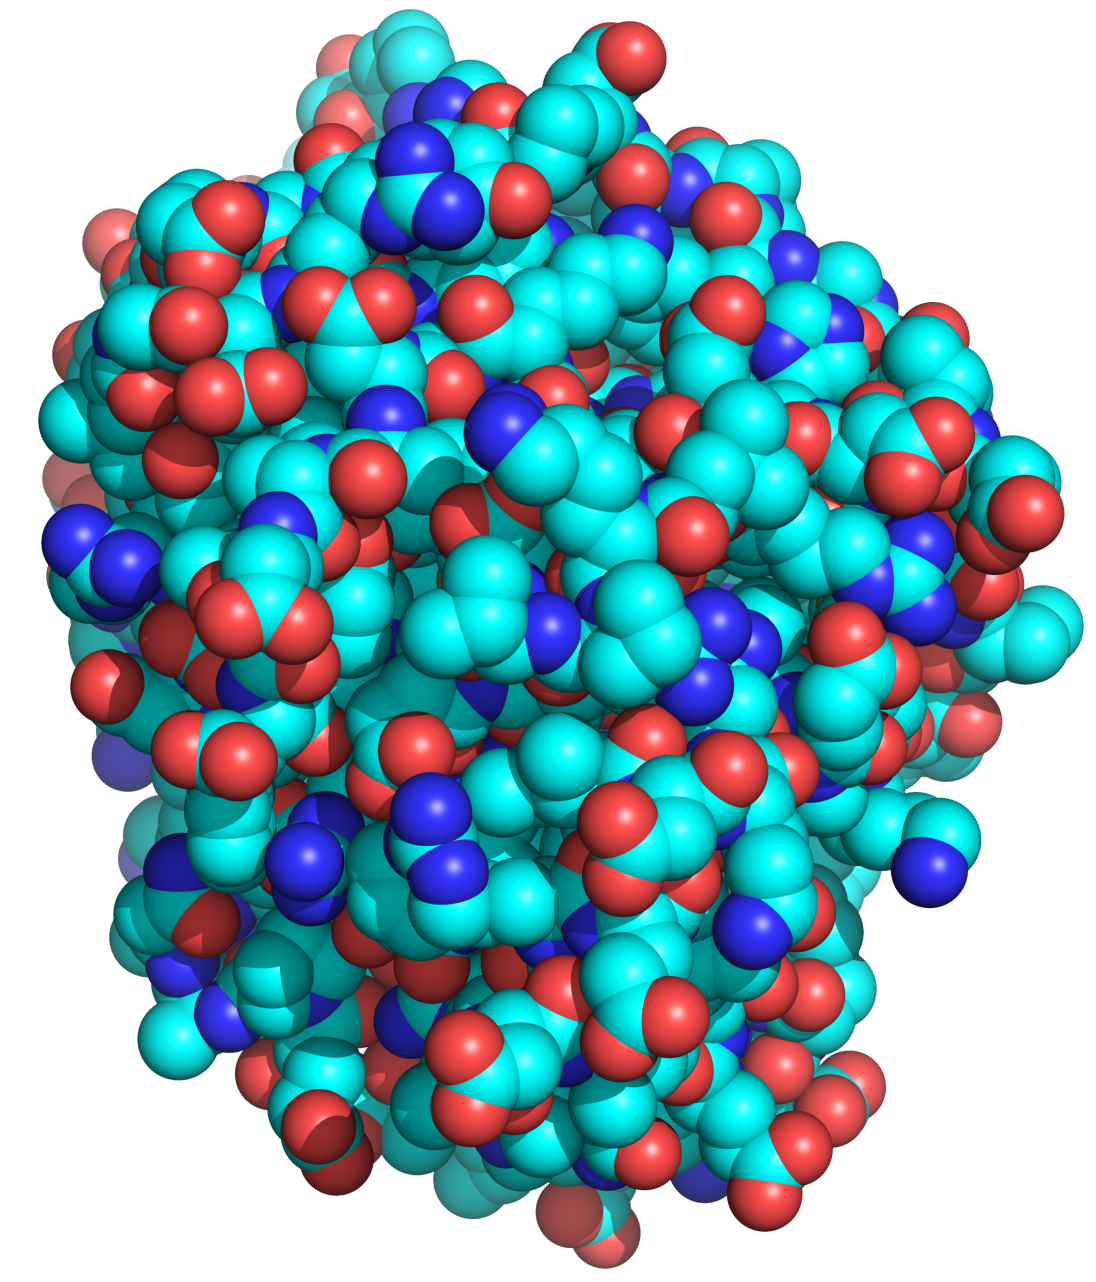
\includegraphics[width=0.17\textwidth]{fig/motiv1} &
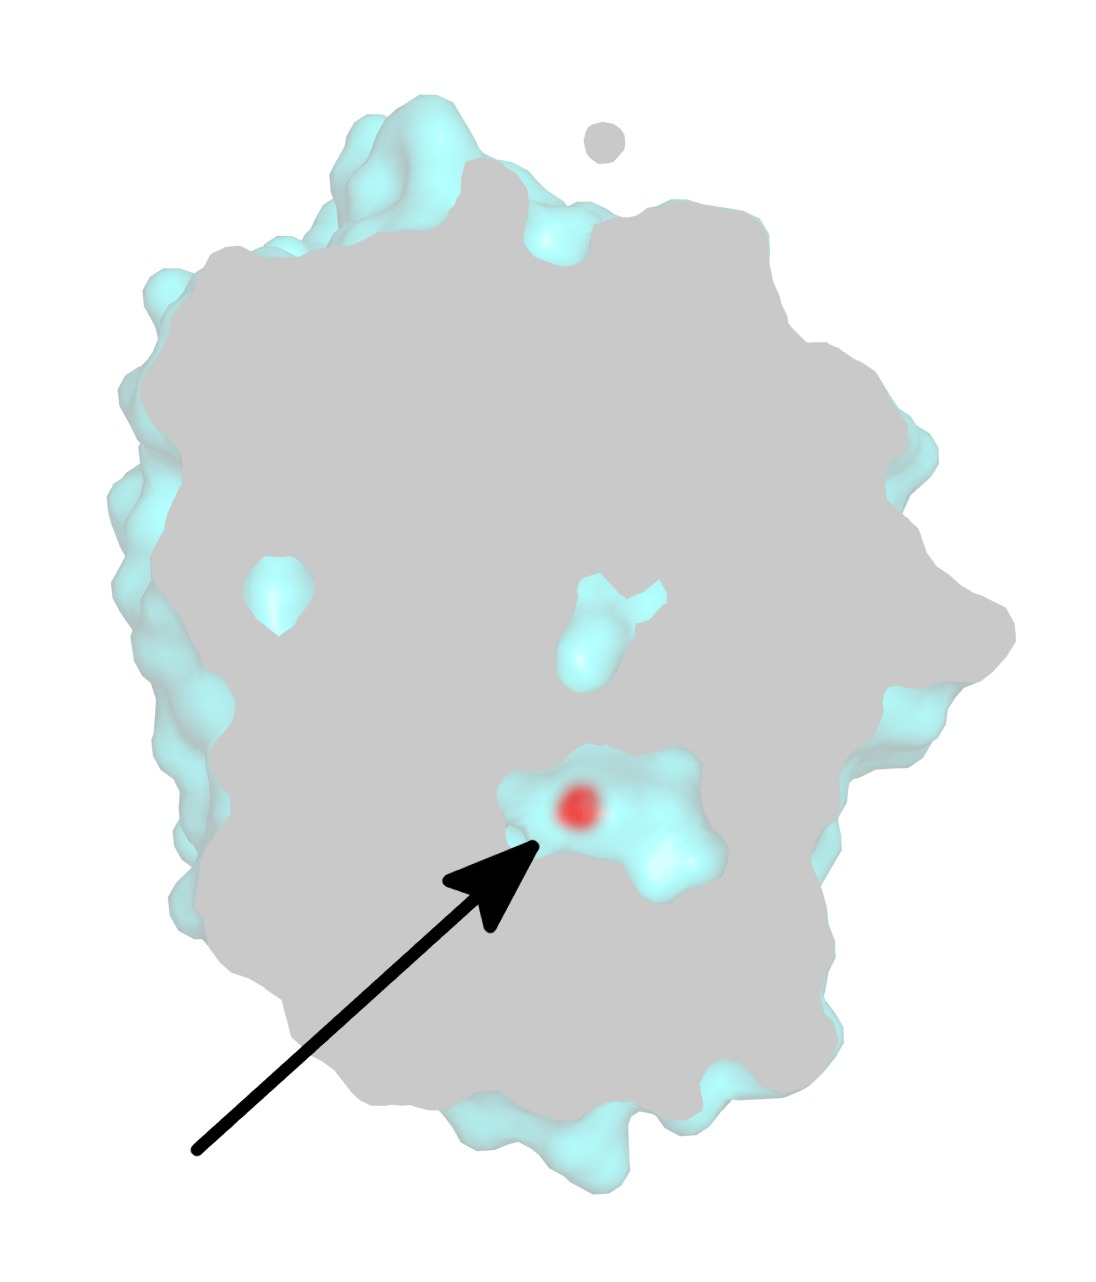
\includegraphics[width=0.19\textwidth]{fig/motiv2lab} \\
Protein 1CQW & Active site \\
\multicolumn{2}{c}{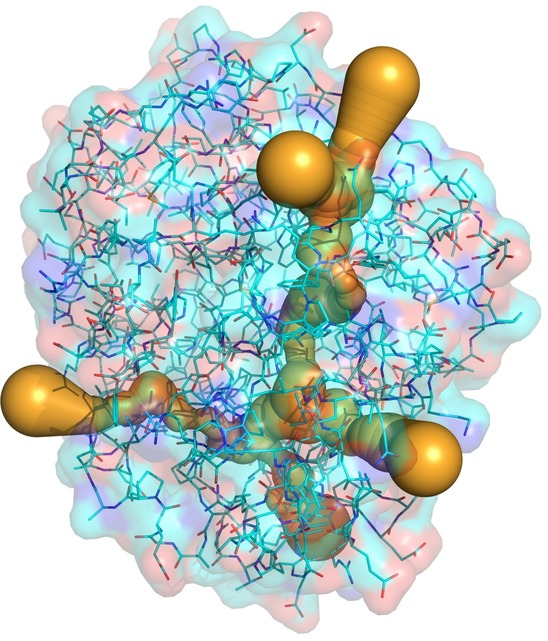
\includegraphics[width=0.19\textwidth]{fig/motiv3}} \\
\multicolumn{2}{c}{Static tunnels }
\end{tabular}
\begin{tabular}{cc}
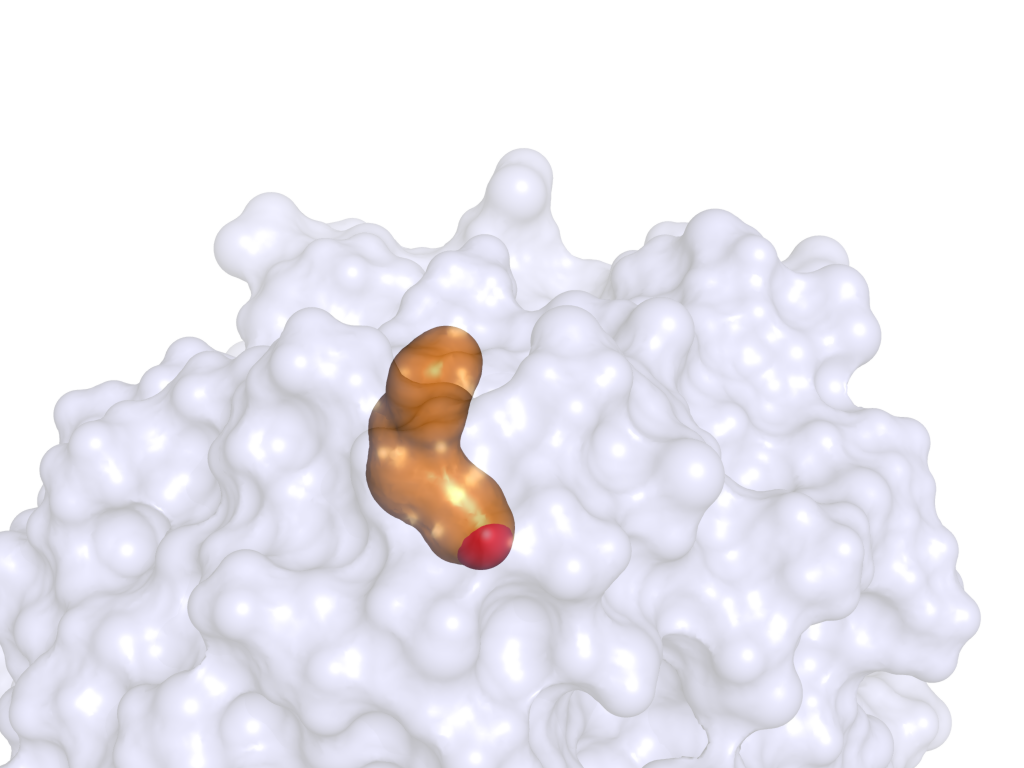
\includegraphics[width=0.26\textwidth]{fig/dt-f5} &
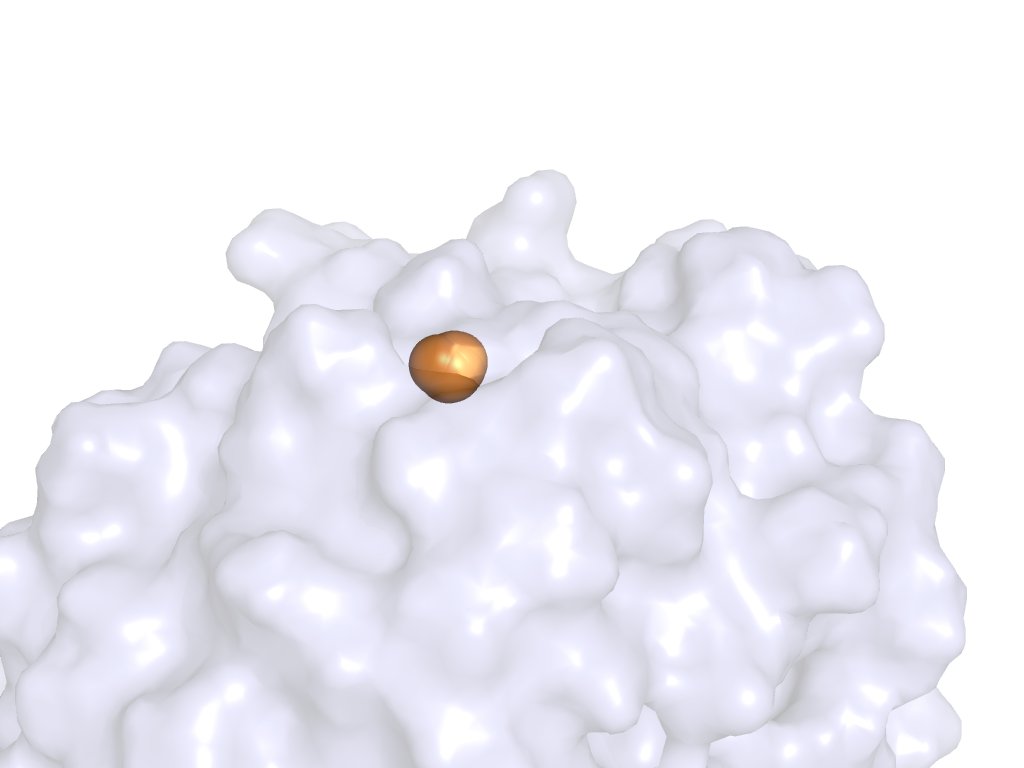
\includegraphics[width=0.26\textwidth]{fig/dt-f6} \\
Frame $i$ & Frame $i+1$ \\
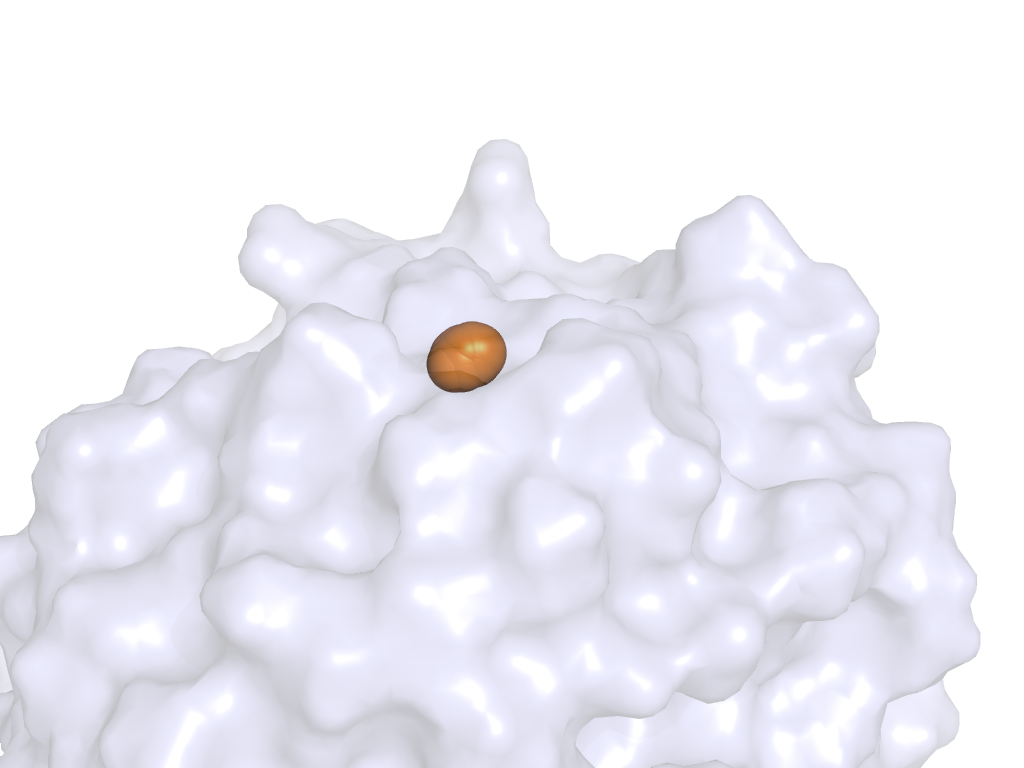
\includegraphics[width=0.26\textwidth]{fig/dt-f7} &
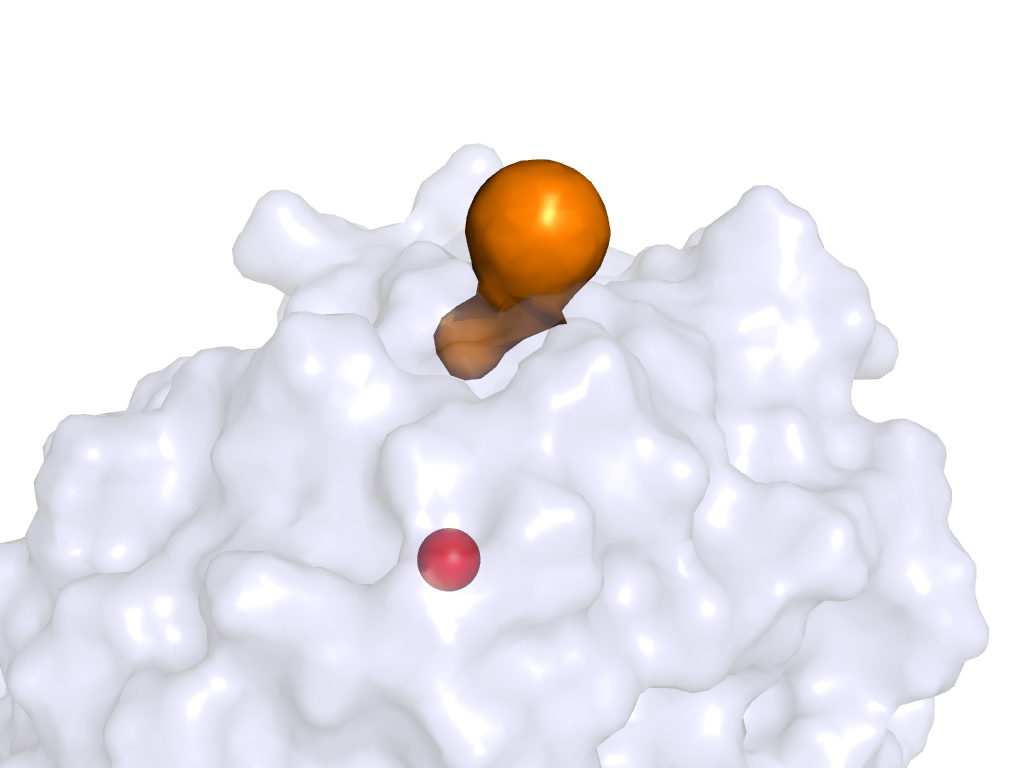
\includegraphics[width=0.26\textwidth]{fig/dt-f8} \\
Frame $i+2$ & Frame $i+3$ \\
\end{tabular}
}
\caption{\label{fig::motiv}
The example of static tunnel detection in the DhaA haloalkane dehalogenase protein and the example of a dynamic tunnel that evolves through four consecutive frames.
In the frame $i$, the active site (red sphere) is not fully connected with the protein surface, but only to the internal cavity.
The cavity is disconnected from the active site in the frame $i+1$ and remains disconnected also in the next frame $i+2$.
In the fourth frame $i+3$, the cavity connects with the protein surface.
}
\end{figure}

Due to the generally low volume of the protein void space, the sampling-based tunnel detection may suffer from the narrow passage problem.
To cope with the narrow passages, we propose to generate the random samples along a subset of Voronoi vertices of the atoms.
The subset is automatically adapted so it always attracts the tree towards the unexplored regions of the configuration space.

%Additionally, we propose a novel approach to the detection of the dynamic tunnels, which solves the second aforementioned problem.

To summarize, the main contributions of this paper are:
\begin{itemize}
\item The novel method for guiding the growth of the tree using multiple regions (defined by Voronoi vertices) that are switched according to the progress of the tree.
\item Introduction of the concept of the dynamic tunnel, enabling to trace the void space behavior over time. Designing the algorithm for its computation.
\item Intuitive visual representations enabling the user to better understand and explore the dynamic tunnels within the MD simulation.
\end{itemize}


%%%%%%%%%%%%%%%%%%%%%%%%%%%%%%%%%%%%%%%%%%%%%%%%%%%%%%%%%%%%%%%%%%%%%%%%%%%%%%%
\section{Related Work}


The analysis of protein structure aiming to reveal tunnels has been supported by different computational software tools, which take the geometry of the protein as an input and explore the inner void space (e.g., MOLE~\cite{Petrek20071357} or CAVER 1.0~\cite{petrek2006caver}).
Early methods for tunnel detection utilized a discretized 3D grid, where each cell was considered as occupied or free depending on the presence of atoms of the protein.
Tunnels can be then searched using standard graph-search methods, such as the Dijkstra's algorithm.
Besides, the grid can be used to identify other relevant properties like pockets, cavities, or channels~\cite{sehnal2013mole,petrek2006caver}.
%One of the first grid-based approaches to the detection of tunnels in protein is the CAVER 1.0 algorithm by Pet\v{r}ek et al.~\cite{citeulike:6257975}.
The obvious disadvantage of the grid-based methods is the high memory demand and their dependency on the grid resolution.
Due to the high memory consumption, these methods are not suitable for tunnel detection in dynamic proteins and therefore they are used primarily for the analysis of static molecules or individual snapshots of the dynamics.

Currently the most widely used approach to tunnel detection is based on ordinary Voronoi diagrams (VD) or Weighted Voronoi diagrams (WVD).
The ordinary VD is computed on points representing centers of all atoms, without considering the atomic radii.
This may lead to the detection of tunnels with incorrect bottlenecks. % i.e., incorrect radius of a smallest probe that can traverse the tunnels.
To consider atoms with different radii, the weights of individual points are determined by the van der Walls radii of the atoms in WVD.
An alternative solution is to compute a non-weighted VD on an extended point set, where each atom is approximated by several spheres with a small radius~\cite{yaffe2008,caver3,caverDetails}.
VD-based methods are memory less demanding, and also faster than the grid-based methods.
The extension of VD-based methods to dynamic molecules requires to construct VD in the frames being analyzed and finding the correspondences between them.
The existing approaches often use hierarchical clustering to match Voronoi vertices and edges from different frames, which is computationally demanding~\cite{lindow2012dynamic,caverDetails}.
Another problem of these approaches is the definition of tunnel bottleneck threshold, which determines the minimal size of the narrowest tunnel point.
If the bottleneck radius is even slightly below this threshold, the tunnel is discarded. 
This leads to the problem of missing tunnels in several or many snapshots of the MD simulation, even when the void space is still present in them.




Alternatively, the tunnel detection in dynamic proteins can be formulated as path planning in 4D (i.e., 3D $\times$ time) configuration space assuming a spherical probe.
This space can be searched using sampling-based motion planning methods like Probabilistic Roadmaps (PRM)~\cite{kavrakiPRM} and Rapidly Exploring Random Tree (RRT)~\cite{lavalleRRT} and their modifications.
In sampling-based motion planning, the configuration space is randomly sampled and the samples are classified as free or non-free using collision detection.
The collision detection is performed between the geometry of the robot (i.e., the probe) and the environment (the atoms of the protein).
The collision-free samples are stored into a roadmap which is searched using standard graph-search methods for a path.
The path in the roadmap then describes a motion in the workspace.

The advantage of sampling-based motion planners is that they can cope with many-DOF (Degrees Of Freedom) robots and due to black-box collision detection, they can also cope with robots of arbitrary shapes.
Beyond robotics, the sampling-based motion planners have been successfully applied to computational biology problems in studies related to protein folding~\cite{bayazit2001ligand,al2012motion,cortes2010simulating,amato2002using,raveh2009rapid,novinskaya2015improving,songPFintro,kirillova2008an}, ligand docking~\cite{cortes2010simulating,latombe1999motion,mollProt}, or analysis of loop motions~\cite{cortes2004geometric}.
In these applications, the molecules are represented as a kinematic chain where joint angles correspond to bonds of the molecules.

%loop motions~\cite{cortes2004geometric},
%protein folding~\cite{amato2002using,raveh2009rapid,novinskaya2015improving,songPFintro},
%protein folding~\cite{raveh2009rapid,novinskaya2015improving},
%or protein folding combined with ligand diffusion~\cite{cortes2010simulating}.
RRT is a single-query motion planning method.
It incrementally builds a configuration tree $\T$ rooted at the initial configuration.
In each iteration of RRT, a random configuration $\qrand$ is generated and its nearest node $\qnear$ in the tree  is found.
A new configuration $\qnew$ is constructed on the line connecting $\qnear$ and $\qrand$ in the distance $\varepsilon$ (straight-line expansion).
If $\qnew$ is collision-free, it is added to the tree.
The algorithm terminates if the tree approaches the goal configuration to a predefined distance.

In~\cite{guieysse2008structure,cortes2010simulating}, RRT is used to compute exit pathways for a flexible ligand leading from an active site to the surface of the protein.
To cope with many-DOF ligands, the RRT-ML~\cite{cortes2007mlrrt} approach is employed as the basic planner in~\cite{cortes2010simulating}.
RRT-ML expands the tree primarily using those DOF that are essential for achieving the motion of the ligand (i.e., rotation
and translation) and it employs the other DOFs (i.e., those that are responsible for conformation changes) if they hinder the growth of the tree.
In~\cite{cortesMD}, the pathway is found for the opposite direction, from the active site towards the protein surface.
The methods~\cite{guieysse2008structure,cortesMD} do not compute all tunnels explicitly, rather a single pathway.

A well known issue of sampling-based planners is the narrow passage problem.
The narrow passage is a small region of the configuration space containing a part of the solution.
As the samples are generated from the uniform distribution in RRT, the probability of placing the samples into the narrow passages is low and therefore, the probability of expanding the tree through a narrow passage is small~\cite{hannaWIS}.
Consequently, many iterations are needed in order to put enough samples into the passages, which increases the computation time.

A possible solution is to estimate the location of narrow passages from the knowledge of the workspace and generate more samples
in the difficult areas.
PRM-based planners can cope with the narrow passage problem by increasing the probability of sampling, e.g., around medial axis~\cite{amatoOBRRT,amato2002using,wilmarthMAPRM}, or even by shifting uniformly generated samples towards the medial axis~\cite{amatoOBPRM} or its approaximation~\cite{hollemanMAPRM}.
Another approach is to estimate difficult regions online, e.g., based on the number of collision-free samples around a given configuration~\cite{overmarsGauss,hsuBridge}.
Generating random samples in difficult regions however does not ensure the construction of a better tree in the case of RRT-based methods.
As RRT builds the tree incrementally, the tree can connect to a region with increased probability of sampling only if the growth of the tree is not blocked by obstacles.
Instead of increasing probability of sampling in all regions at once, e.g., along the whole medial axis, the tree has to be guided through the space to reach the regions gradually.
For example, the random samples are generated from multiple regions, that are switched according to the progress of the tree.
In~\cite{kardossRRTKK}, the samples are generated along several waypoints that are located close to narrow passages.
A more general approach is to define a guiding path in the workspace and sequentially increase the probability of sampling along the path~\cite{vonasek2009rrt,denny2014marrt,denny2016dynamic}.
%The guiding path can be computed e.g. using medial axis of the worskpace~\cite{denny2014marrt,denny2016dynamic}.

%RRT-based planners cannot cope with the narrow passage problem simply by increasing the probability of sampling in them, as the
%growth of the configuration tree towards the random samples may be blocked by obstacles~\cite{vonasekphd}.
%To prevent blocking of the tree growth by the obstacles, DD-RRT~\cite{yershovaDDRRT} limits the selection of nodes for the expansion to a small ball. 
%The radius of the ball is set to infinity for new nodes, and decreases to a predefined radius if the node cannot be successfully expanded.
%The disadvantage of DD-RRT is the sensitivity to the predefined radius.
%Therefore, the authors of ADD-RRT~\cite{jailletADRRT} proposed to adapt the ball radius according to the success rate of the expansion.
%To attract the tree towards a given region, random samples have to be generated there only if the tree can expand to this region.
%In~\cite{kardossRRTKK}, the probability of sampling is increased in several waypoints close to narrow passages, but without specifying
%the method to find these waypoints.
%The generalization of~\cite{kardossRRTKK} is the guided sampling, where a whole path is used
%to generate samples in the configuration space.
%The path can be computed in the workspace~\cite{vonasek2009rrt}, or iteratively refined in the configuration space based on the solution of a relaxed version of the problem~\cite{bayazitIRC}.
%
%rrt for molecular: \cite{al2012motion}
%survey \cite{gipson2012computational}


\section{Algorithm Overview}

The proposed algorithm works as follows.
In each frame of the protein dynamics, first the void space is detected and represented by a set of spheres connected to a tree structure.
To detect the void space, it is necessary to explore the internal parts of the protein and decide which of them are reachable from a given region (active site) or a set of regions (the void space from the previous frame).
This leads to the incremental exploration of the void space, which can be realized using the RRT principle.

After a void space is detected in a given frame, it is transferred to the next frame and pruned in order to remove collisions with the atoms in the next frame.
During the void space detection, the exit points from the void space to the surface of the protein are detected.
The existence of the exit points indicates the end of either a static or a dynamic tunnel.
If the exit point can be connected with the active site in the given frame, the static tunnel can be reconstructed.
This corresponds to the tunnel detected by traditional methods.
Otherwise, the detected void space is searched back in time to reconstruct our newly proposed dynamic tunnel.

The work presented in this paper is the extension of our previous work~\cite{vonasek2017tunnel}, which proposed to guide the search
of the configuration space using the Voronoi vertices of the Voronoi-based protein representation.
Our goal was to detect static tunnels in proteins.
In this work, we focus on the detection of dynamic tunnels and their visual representation enabling the domain experts to further analyse the evolution and behavior of the protein void space.

\section{Used Notation}

Molecular dynamics simulation is represented by a sequence of consecutive snapshots (frames), where each snapshot describes the position of all protein atoms in a specific time.
Proteins are represented by the hard sphere model, where the radius of each sphere (atom) is given by its van der Waals radius.
The geometry of the protein in the $i-$th frame is represented by the union of all spheres $\SS^i \subset \R^3$.
The void space is detected using the spherical probe of radius $\probe$. 
All possible configurations $q=(x,y,z)$ (positions) of the probe in the $i$-th frame form the configuration space $\C^i$.
The probe is represented by a sphere $\Sprobe(q) \subset \R^3$ at a configuration $q$.
The void space (the collision-free region) $\CF^i \subseteq \C^i$ is formed by configurations, where $\Sprobe$ can be placed without any collision with atoms, i.e.,  $\CF^i = \{q \in \C^i | \Sprobe(q) \cap \SS^i = \emptyset\}$.
For each configuration $q\in\C^i$ we assume that its largest collision-free radius $r(q) \in \mathbf{R}, r(q)\ge 0$ can be computed, e.g., 
using collision detection.
The outer space  $\CG^i \subset \CF^i$ of the protein is defined by configurations, where a large sphere can be placed without any collision,
i.e., $\CG^i=\{q\in \C^i| \Sgprobe(q) \cap \SS^i = \emptyset \}$ where $\Sgprobe$ is the sphere of radius $\gprobe > \probe$ 
placed at the configuration $q$.
The exit points, where the tunnels leave the protein, are located in $\CG^i$.
To determine whether two configurations $q_1, q_2 \in \CF^i$ can be connected, a line segment from $q_1$ to $q_2$ is constructed
and discretized to several points, using $\varepsilon$ discretization step, and the collision detection is performed at all the points.
The two configurations can be connected if all intermediate points on the line are collision-free. 
The 3D Euclidean metric is used to measure distances in the configuration space.

The main purpose of the tunnel detection is the identification of tunnels, either static or dynamic, that connect the active site with the protein surface.
We assume that the position (configuration) of the active site $\qinit \in \CF^i$ in each snapshot is known in advance or it is known that the probe cannot be placed at the active site.
A static tunnel is a collision-free path leading from $\qinit \in \CF^i$ to an exit point $q \in \CG^i$, i.e., both active site and the exit point are located in the same frame $i$.
A dynamic tunnel is a collision-free path leading from $\qinit \in \CF^i$ to an exit point $q \in \CG^j$, $j>i$, i.e., the active size and the exit point are located in different frames.

The approximated WVD diagram of the atoms is computed by representing each atom using 12 balls of equal radii and computing the ordinary Voronoi diagram.
Computing WVD this way is numerically more stable and it is used also in other related tools~\cite{caver3,yaffe2008}.
The vertices of this WVD are filtered out if their distance to an atom is less than the probe radius $\probe$ or if their distance to the nearest atom is larger than $\gprobe$.
These filtered Voronoi vertices are stored in the set $\VV^i$.
The atoms located on the surface of the molecule can be identified using \mbox{$\alpha$-shape} with radius $\gprobe$.
Let $\SSA^i \subset \SS^i$ denote a set of spheres representing these atoms in snapshot $i$.


\section{Void Space Detection in a Single Frame} 

To detect the void space, the collision-free region $\CF^i$ of the $i$-th frame is searched and represented as a tree structure of the collision-free configurations.
The detection starts from a given active site $\qinit \in \CF^i$ or from a set of already detected collision-free positions of the probe.
The second case is a result of the void space detection in the previous frame of the molecular dynamics.
To maintain the connectivity between the void space from the previous frame and the newly discovered one (i.e., from $\CF^i$ to $\CF^{i+1}$, the void space has to be explored incrementally without adding non-reachable regions, such as cavities.
Due to this reason, the void space cannot be automatically initialized using all Voronoi vertices $\VV^i$, though they are collision-free at the radius $\probe$, because the Voronoi vertices can be also placed in the cavities.
The required incremental detection of the void space can be achieved by the exploration principle of the RRT planner, as RRT incrementally extends a tree of collision-free configurations.
The main loop of the algorithm for the void space detection is listed in Alg.~\ref{alg::main}. 

We propose three modifications of the RRT for the purpose of void space detection.
The aim of the first modification is to prevent the tree to grow outside the protein. 
This is necessary in order to achieve the void space detection only inside the protein.
The second modification is introduced to generate the random samples around the Voronoi vertices of the protein.
This helps to build the tree inside the narrow void space in a smaller number of iterations.
Finally, we modify the expansion step of the RRT planner in order to build denser trees.
These three modifications are described in detail in the following subsections.

\linesnumbered
\begin{algorithm}[h]
%\setstretch{\straa}
{\small
\caption{\label{alg::main}voidSpaceDetection}
\KwIn{Initial configuration tree $\T$,
    initial set of blocking spheres $\SB'$,
    position of active site $\qinit\in\CF^i$,
}
\KwData{goal-probe radius $\gprobe$,
    probe radius $\probe$, 
    number of iterations $\Imax$, 
    phase--switching parameter~$\alpha$,
    prob. $\gb$~of sampling randomly from~$\C^i$,
}
\KwOut{Configuration tree $\T$,
    list of tunnel exit-points $P$
}
\hrule
$\SB = \SB'$; //blocking atoms added during phase~1 \\
$P = \emptyset$; // list of tunnel exit-points \\
$phase=1$\;
$\VV^i = \VV^i \cup \{ \qinit \}$; // add active site position in order to reach it by the tree\\
updateCollisionDetection($\SB$)\;       
\For{$iteration = 1:\Imax$}{
    \If(// Voronoi-based sample --- Section~\ref{sec::vbg}){$phase=1$}{
        $\VVA^i$ = updateActiveVoronoiVertices($\T, \VV^i$)\;
        $\VVA^i$ = sort vertices according to the distance to the tree\; \nllabel{alg::main::d}
        \ForEach{$v \in \VVA^i$}{
            $\qnear$ = nearestNode($\T, v$)\;
            $\T,P', \SB'$ = expandTree($\T, \qnear, v$)\;
            $P = P \cup P'$\; \nllabel{alg::main::g1}
            $\SB = \SB \cup \SB'$\;
            updateCollisionDetection($\SB$)\; \nllabel{alg::main::a} \nllabel{alg::main::e}
        }
    }
    \If{$phase=1$}{ \nllabel{alg::main::f}
        $v =$ random point from $\VVA^i$\;
        $\qrand =$ random point $\sim N(v,r_v)$\; \nllabel{alg::main::gauss}
    }
    \If{$phase=2$ {\bf or} rand(0,1) $< p_c$}{
        $\qrand$ = random sample from $\C^i$\; \nllabel{alg::main::rand}
    }

    $\qnear$ = nearestNode($\T, \qrand$)\;
    $\T,P',\SB'$ = expandTree($\T, \qnear, \qrand$)\;
    $P = P \cup P'$\; \nllabel{alg::main::g2}
    $\SB = \SB \cup \SB'$\;
    updateCollisionDetection($\SB$)\; 

    \If{$phase = 1$ {\bf and} $iteration > \alpha \Imax$}{ \nllabel{alg::main::b}
        $phase = 2$\;
        removeFromCollisionDetection($\SB$)\;
        $\SB = \emptyset$; // block. atoms are not used in phase 2 \\
    }
}
\return $(\T, P)$\; 
}
\end{algorithm}


\subsection{Protection from Sampling the Protein Outer Space}

Besides the exploration of the void space, it is necessary to detect the exit points as well.
The exit points are configurations from $\CG^i$, i.e., they are collision-free at the radius $\gprobe$ and they define the end of the tunnel.
The detection of the exit points requires that the tree exits the protein.
A premature exit from the protein may lead to quick filling of the outer part of the protein and eventually even to entering the protein from outside. 
Such an exploration would lead to the detection of a smaller number of tunnels.
The example is depicted in Fig.~\ref{fig::blocking1}.

To ensure that the tree explores primarily the internal void space while allowing its growth outside the protein for the purpose of exit point detection, the algorithm is divided into two phases.
In the first phase, the growth of the tree outside the protein is blocked using a set of {\sl blocking spheres} $\SB$.
The blocking spheres are placed at configurations that are located close to the surface atoms $\SSA^i$.
After a configuration $q$ is added to the tree, the distance between $q$ and the surface atoms is computed.
If the distance is smaller than a predefined threshold $\dts$, $q$ can be assumed to be close to the surface and a new blocking sphere of radius $\gprobe$ is added to $\SB$.
By adding the blocking sphere at $q$, the tree cannot further expand not only from $q$, but also from the nearby nodes, which ensures that the tree will not exit the protein in the first phase of the void space detection.

In the second phase, the blocking spheres are not used and they are removed from the collision detection (Alg.~\ref{alg::main}, line~\ref{alg::main::b}).
This allows the tree to explore also the void space outside the protein, which is necessary to find configurations representing the tunnel exit points.
The outer space is more likely reached from the nodes that could not be expanded in the first phase due to the blocking spheres.
As these nodes are located close to the surface atoms, this situation does not require many iterations to expand these nodes.
The second phase of the algorithm should therefore be shorter than the first one.
In Alg.~\ref{alg::main}, the second phase starts after $\alpha$ fraction of the iterations.

\begin{figure}
\centering
{
\renewcommand{\tabcolsep}{1pt}
\begin{tabular}{cccc}
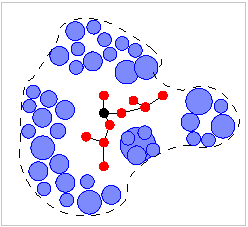
\includegraphics[width=0.24\textwidth]{fig/blockingb1} &
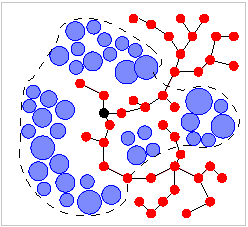
\includegraphics[width=0.24\textwidth]{fig/blockingb2} & 
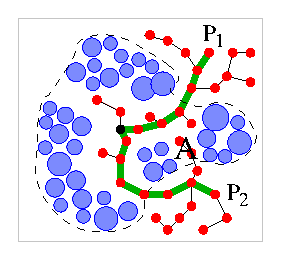
\includegraphics[width=0.24\textwidth]{fig/blockingb3} & 
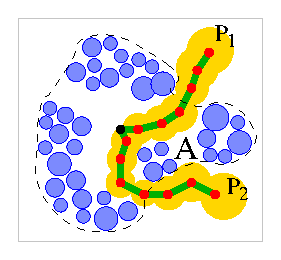
\includegraphics[width=0.24\textwidth]{fig/blockingb4} \\
a & b & c & d \\
\end{tabular}  
}
\caption{\label{fig::blocking1}
    Example of the tree growth without the blocking spheres. 
    The initial configuration $\qinit$ (active site) is represented by the black circle.
    The tree starts to grow inside the protein (a) but it can grow outside as well (b).
    In region denoted by A, the tree grows back to the protein (c).
    Finally, two tunnels are detected (with the exit points $P_1$ and $P_2$), but any tunnel is found in the region $A$ (d).
}
\end{figure}

\begin{figure}
\centering
{
\renewcommand{\tabcolsep}{1pt}
\begin{tabular}{cccc}
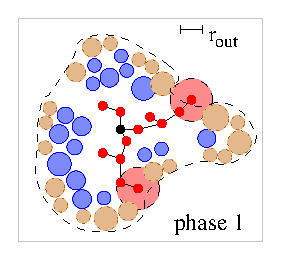
\includegraphics[width=0.24\textwidth]{fig/blockingb5} &
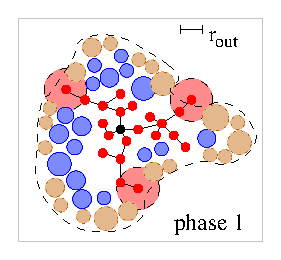
\includegraphics[width=0.24\textwidth]{fig/blockingb6} &
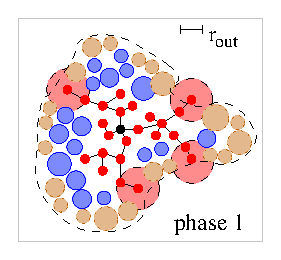
\includegraphics[width=0.24\textwidth]{fig/blockingb7} & 
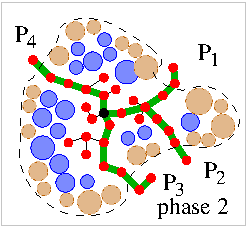
\includegraphics[width=0.24\textwidth]{fig/blockingb9} \\
a & b & c & d \\
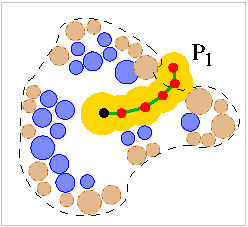
\includegraphics[width=0.24\textwidth]{fig/blockingb10a} &
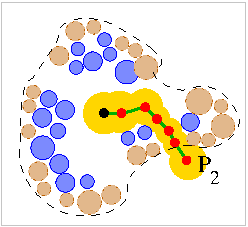
\includegraphics[width=0.24\textwidth]{fig/blockingb10b} & 
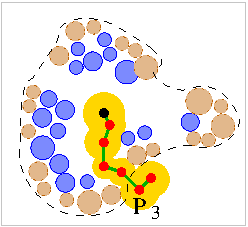
\includegraphics[width=0.24\textwidth]{fig/blockingb10c} & 
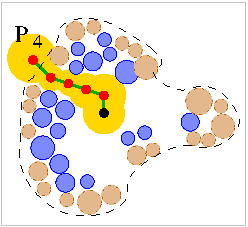
\includegraphics[width=0.24\textwidth]{fig/blockingb10d} \\
e & f & g & h \\
\end{tabular}
}
\caption{\label{fig::blocking2}
The effect of the blocking spheres. 
The surface atoms are depicted in brown.
After the tree reaches a surface atom, a new blocking sphere (red large circle) of size $\gprobe$ is added to the collision detection (a).
This forces the tree to explore only the internal void space (b,c).
In the second phase of the algorithm, the blocking spheres are removed and the tree can finally grow outside the protein in order
to detect exit points (d).
Figures e--h depict four detected tunnels.
}
\end{figure}


\subsection{Voronoi-Based Guided Sampling}
\label{sec::vbg}

The generation of the random samples directly influences the performance of the RRT-based planners.
In classic RRT, the random samples are drawn uniformly in the whole configuration space, which leads to the well known narrow passage problem.
The void space can be considered as a narrow passage, as the movement of the probe is constrained by many atoms.
The limitation is even higher for larger probes.
To boost the growth of the tree inside the narrow void space, the random samples can be generated around places that are believed to be a part of the collision-free region $\CF^i$.
This region is approximated by the Voronoi vertices $\VV^i$ and the random samples can be generated around them.

However, the probability of sampling cannot be increased around all Voronoi vertices at once, because the growth of the tree towards the Voronoi vertices may be blocked by the obstacles (atoms)~\cite{vonasekphd}.
It is necessary to guide the growth of the tree by increasing the probability of sampling only around such Voronoi vertices that can be reached by the tree with a higher probability.
Such Voronoi vertices have to be located close to the tree.
Therefore, a subset $\VVA^i \subseteq \VV^i$ of the Voronoi vertices that are close to the tree is maintained (Alg.~\ref{alg::update}).
A Voronoi vertex $v \in \VV^i$ is considered as active if the distance to its nearest node in the tree is less than $\da$, but larger than
$\db$.
After the update of $\VVA^i$, the tree attempts to expand towards them (Alg.~\ref{alg::main}, line~\ref{alg::main::d}--\ref{alg::main::e}).
This expansion is not always successfull, especially for distant Voronoi vertices, but it helps the tree to explore the void space.


\begin{algorithm}
{\small
\caption{\label{alg::update}updateActiveVoronoiVertices}
\KwIn{configuration tree $\T$, 
    Voronoi vertices $\VV^i$,
}
\KwData{
    minimum distance to the tree $\da$, 
    maximum distance to the tree $\db$
}
\KwOut{
    set $\VVA^i$ of active Voronoi vertices
}
\hrule
$\VVA^i = \emptyset $\;
\ForEach{$v \in \VV^i$}{
    $d$ = nearestNode($\T, v$)\;
    \If{$\db \le d \le \da$}{
        $\VVA^i = \VVA^i \cup \{ v \}$\;
    }
}
\return $\VVA^i$
}
\end{algorithm}




\begin{figure}
\centering
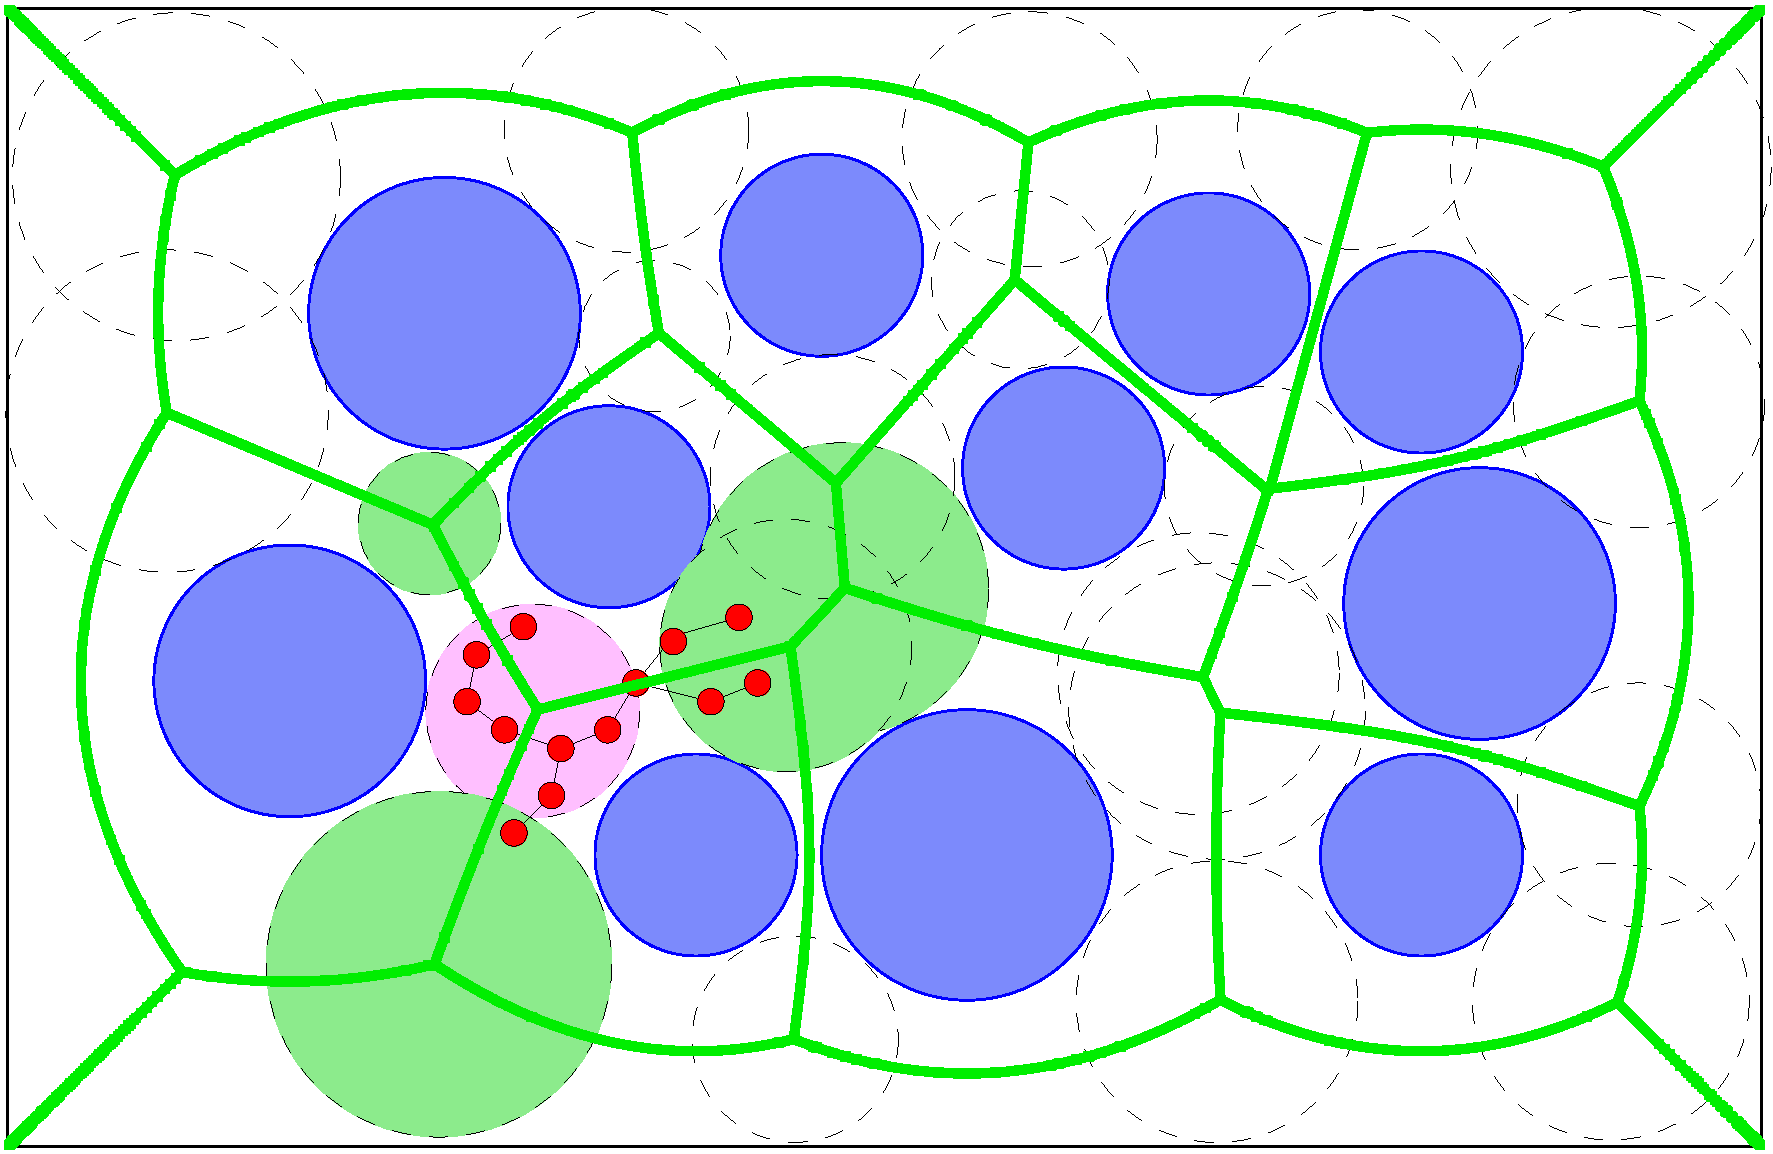
\includegraphics[width=0.4\textwidth]{fig/activevor}
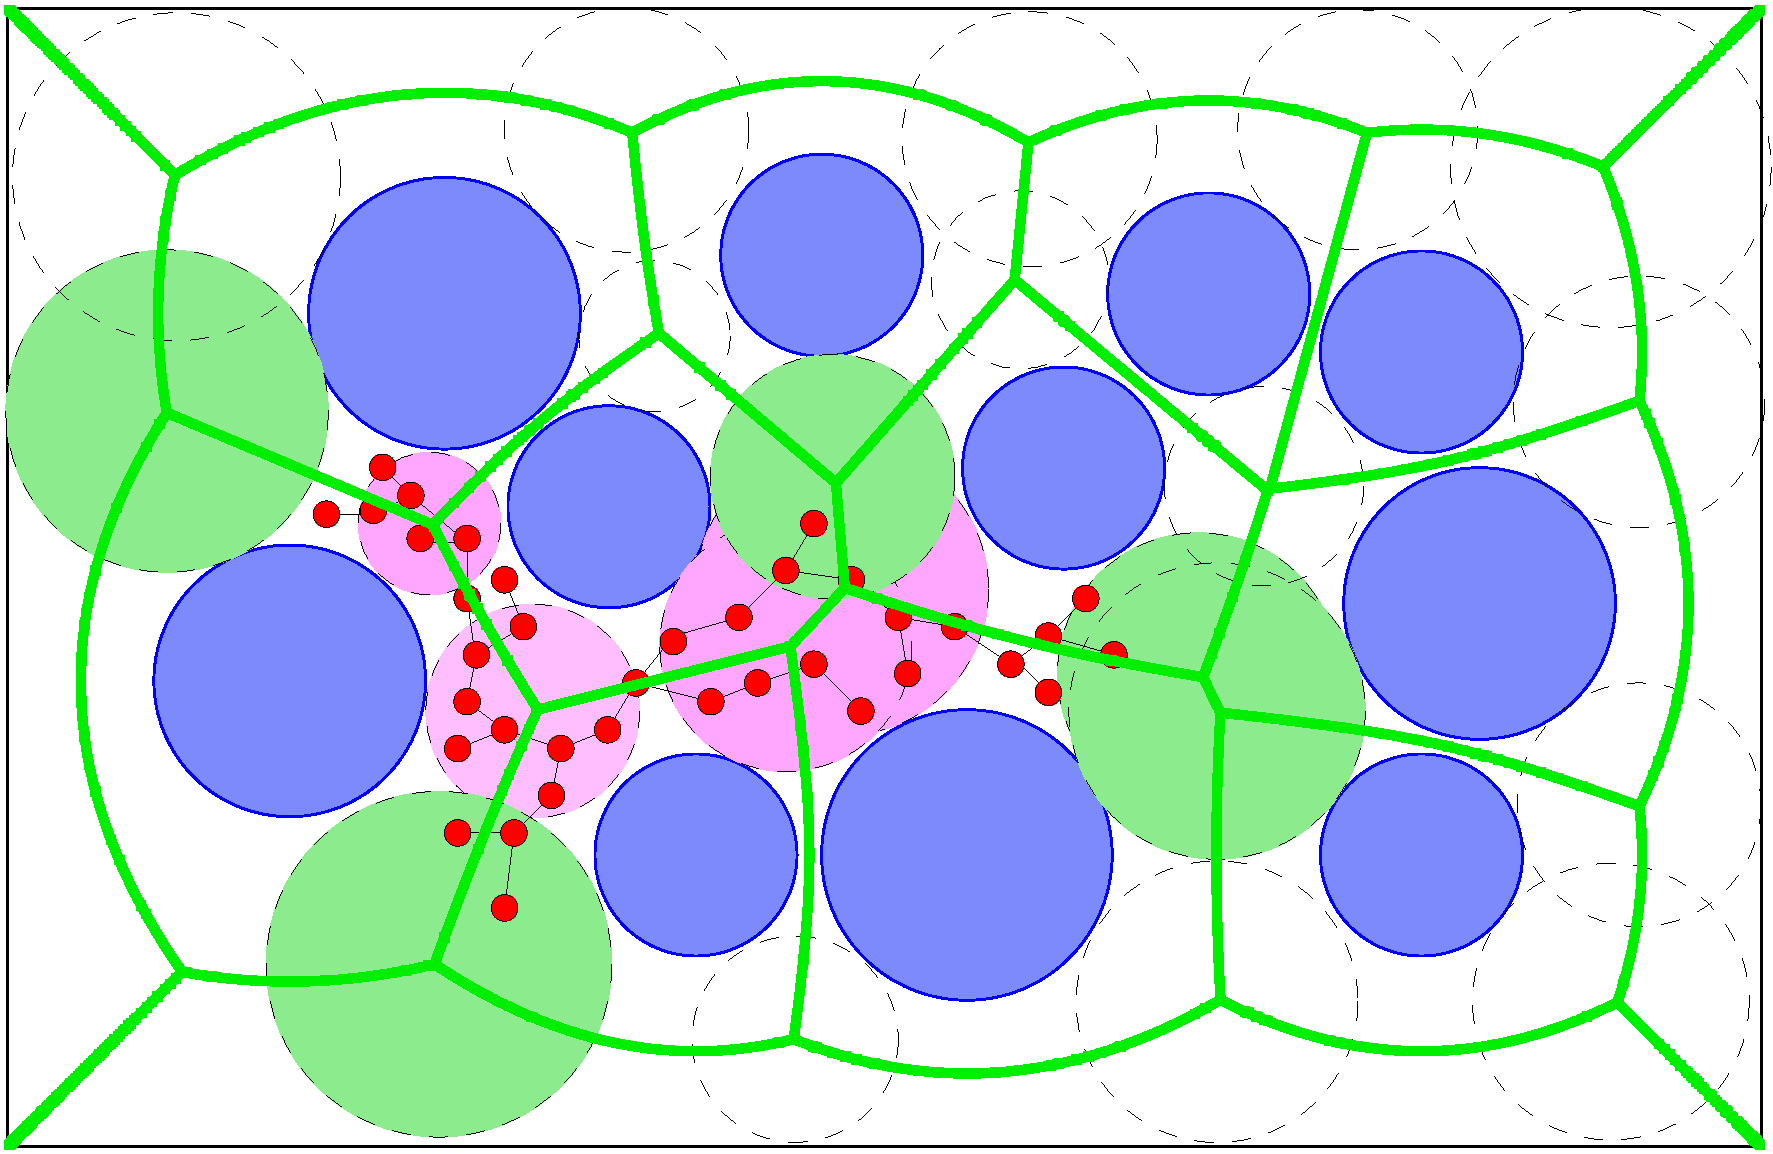
\includegraphics[width=0.4\textwidth]{fig/activevor2}
\caption{\label{fig::av}
    A simplified example of the progress of generating random samples using WVD for a set of atoms in 2D.
    The atoms are depicted in blue, the WVD edges in green.
    The dashed circles are centered at Voronoi vertices, and their radii are given by the distance to the nearest atom.
    The small red circles represent a partially built configuration tree.
    The active Voronoi vertices that are close to the tree are depicted in green.
    The random samples are generated around these active vertices.
    The tree is attracted by the samples in the green regions (left). 
    After several iterations, the tree reaches the Voronoi vertices close enough, so they are removed from the active Voronoi set. 
    A new set of Voronoi vertices is activated (green) and the tree continues to reach them (right).
}
\end{figure}



In the first phase of the algorithm, where the tree growth outside the protein is blocked, the random samples are generated mainly around the active Voronoi vertices (Alg.~\ref{alg::main}, line~\ref{alg::main::f}).
To generate a random sample $\qrand$, $v \in \VVA$ is randomly selected and $\qrand$ is generated around $v$ using the Gaussian distribution with  $\sigma = r_v$ (Alg.~\ref{alg::main}, line~\ref{alg::main::gauss}).
In the second phase, the tree is required to grow outside the protein and therefore, the random samples are generated from the whole configuration space (Alg.~\ref{alg::main}, line~\ref{alg::main::rand}).


By maintaining the active Voronoi vertices $\VVA^i$, the random points are automatically generated around the borders of the configuration tree (Fig.~\ref{fig::av}).
As the Voronoi vertices are located inside the protein, generating random samples around them further boosts the search of the internal void space.
After the tree approaches a vertex $v \in \VVA$ too close (less than the distance $\db$), the vertex is removed from $\VVA^i$ in the next update, and the random samples are not generated around it.
The upper value $\da$ determines how far from the tree are the random samples generated, while $\db$ prevents to generate
the random samples around Voronoi vertices, that have already been approached by the tree.
The visualization of the tree growth towards the active Voronoi vertices is depicted in Fig.~\ref{fig::1akdvv}.

\begin{figure}
\centering
{
\renewcommand{\tabcolsep}{1pt}
\begin{tabular}{cc}
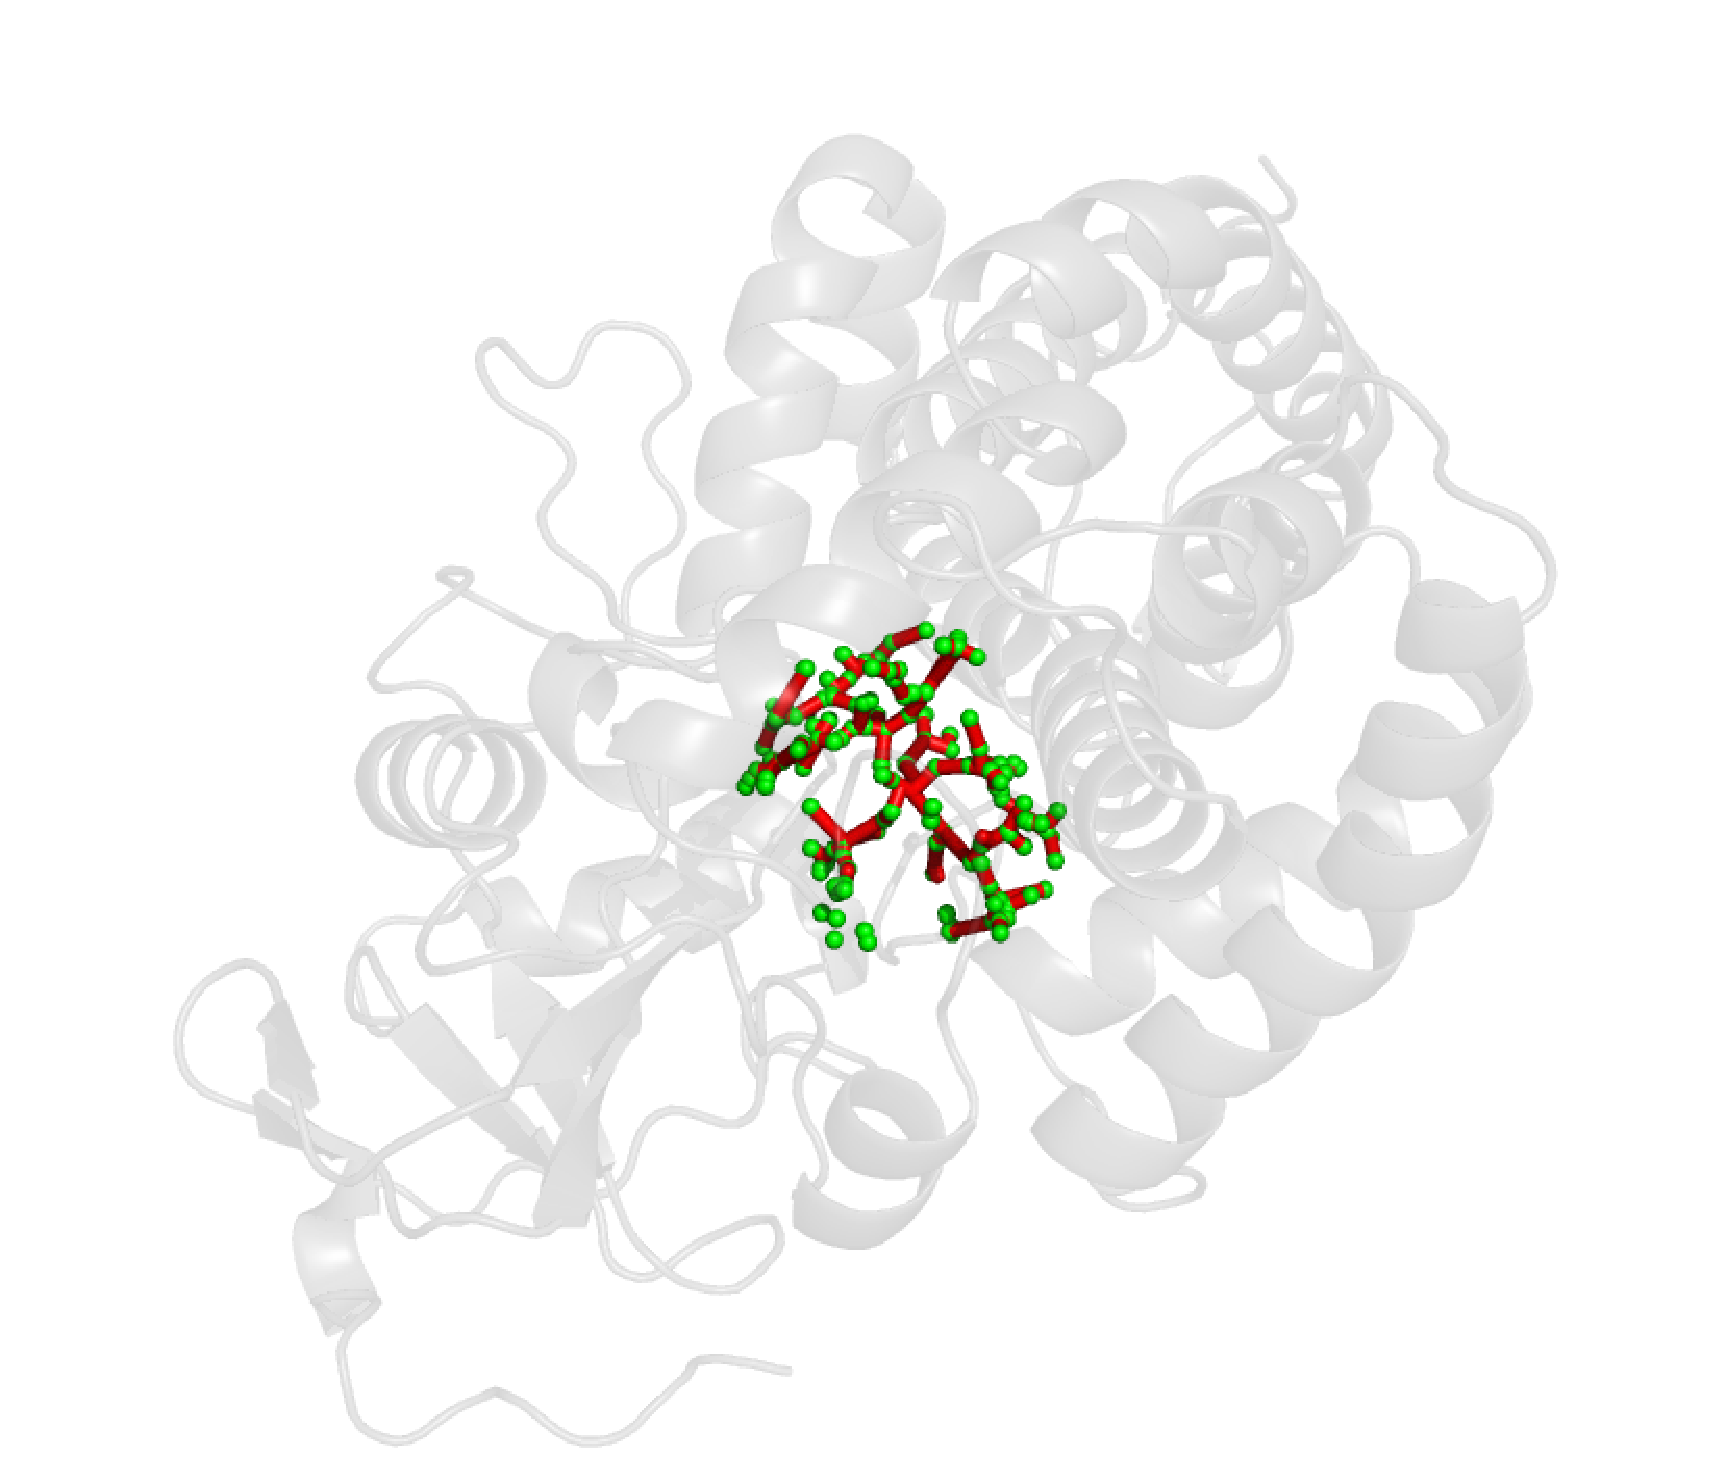
\includegraphics[width=0.45\textwidth]{fig/1akd2-0} &
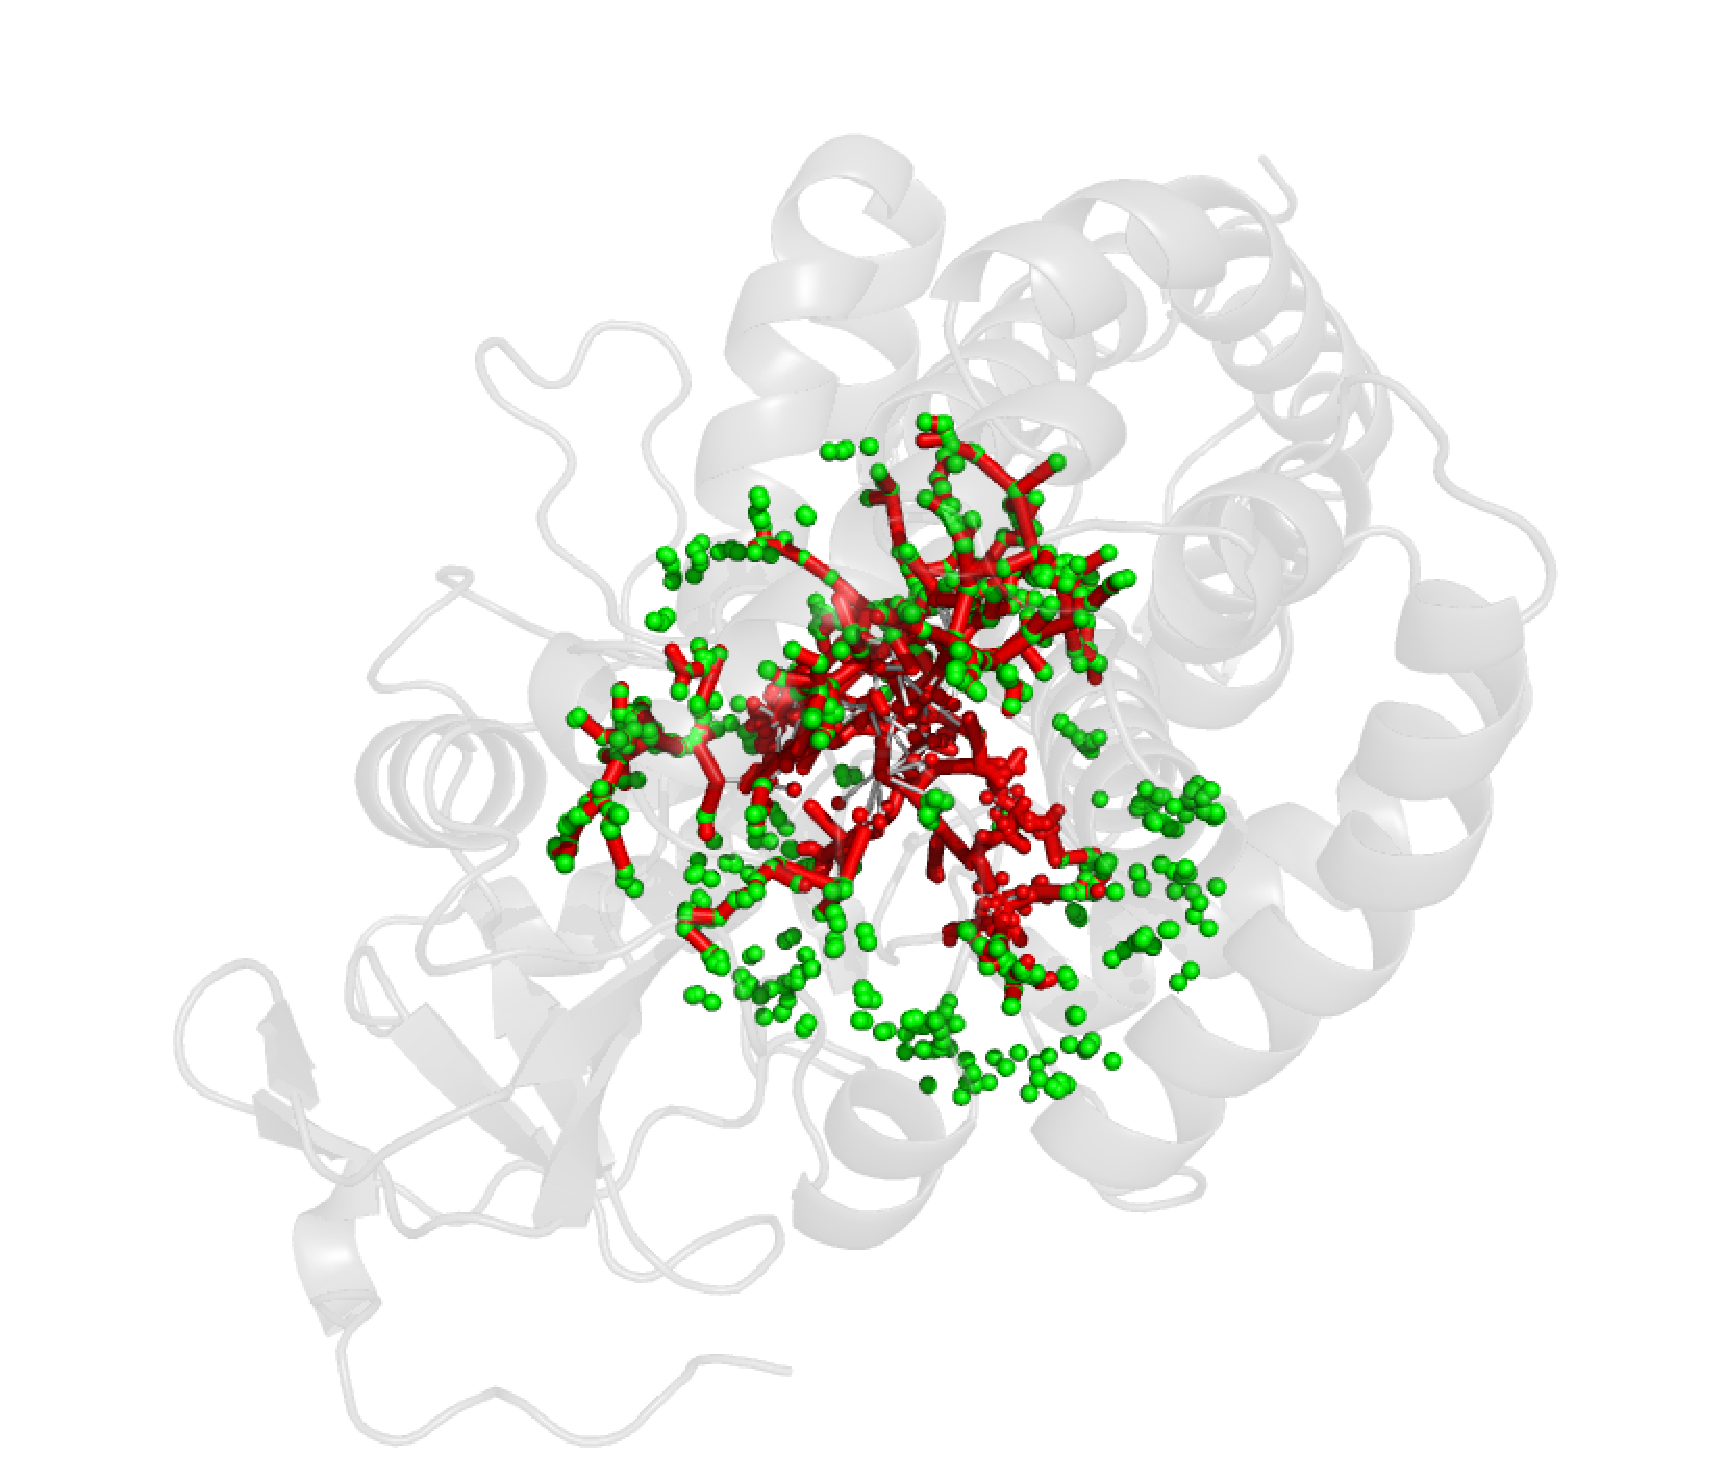
\includegraphics[width=0.45\textwidth]{fig/1akd2-41} \\
Iteration 100 & Iteration 400 \\
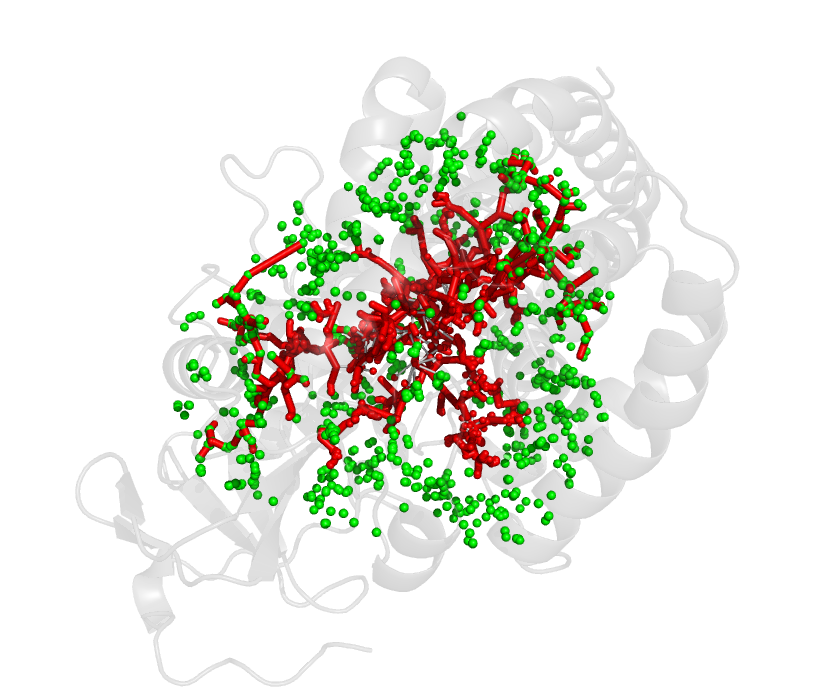
\includegraphics[width=0.45\textwidth]{fig/1akd2-102} &
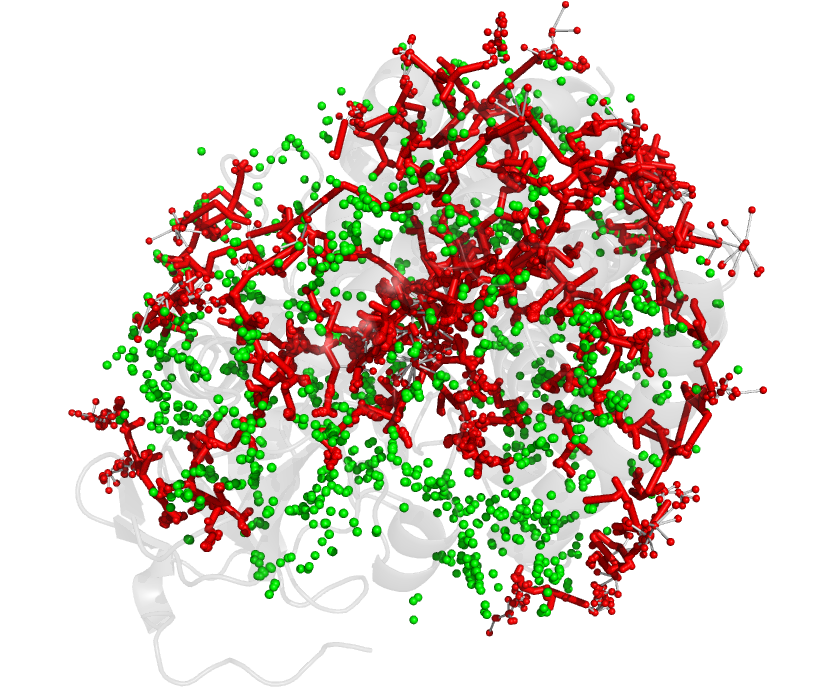
\includegraphics[width=0.45\textwidth]{fig/1akd2-10k} \\
Iteration 1000 & Iteration 10000 \\
%\multicolumn{2}{c}{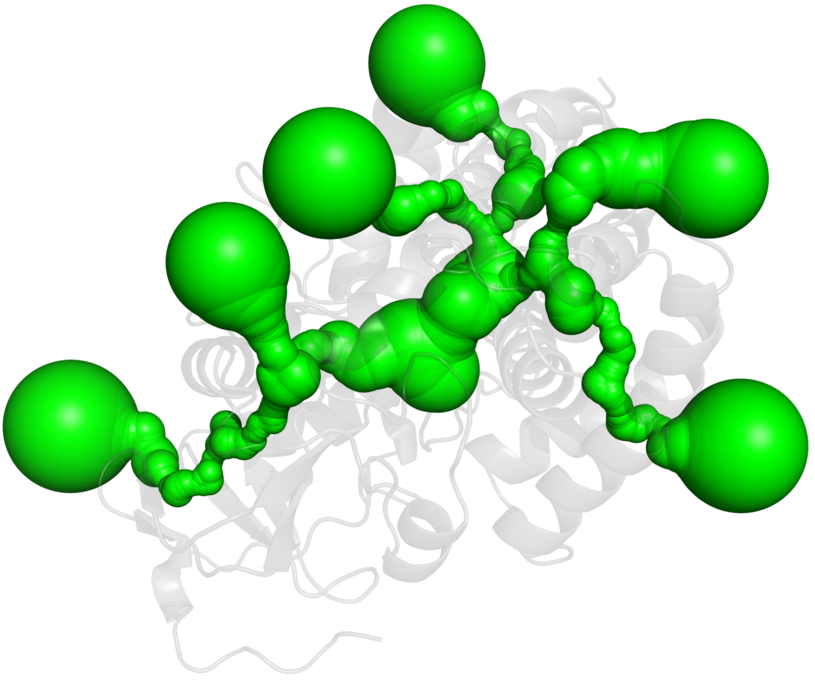
\includegraphics[width=0.45\textwidth]{fig/1akd2-tunnels2}} \\
%\multicolumn{2}{c}{Detected tunnels}
\end{tabular}
}
\caption{\label{fig::1akdvv}
    Example of the tree growth in the protein with PDB ID 1AKD.
    The active Voronoi vertices are depicted in green and the tree is depicted in red.
    After the tree reaches these vertices to the distance $\db$ ($\db=1$~\AA\ in this case), the vertices are disabled.
}
\end{figure}


\subsection{Expansion of the Tree}

The tree expansion is the crucial part of the RRT-based planners.
In the case of protein void space, which possesses the properties of narrow passages, it is suitable to expand the tree not only by one node, as it is suggested in the original RRT, but using multiple nodes at once.
Expanding the tree by multiple nodes leads to a faster exploration of narrow passages, because by placing more samples there, the probability of successful expansion inside the narrow passages increases.

\begin{figure}
\centering
{
\renewcommand{\tabcolsep}{3pt}
\begin{tabular}{ccc}
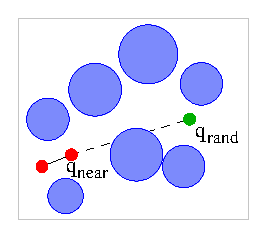
\includegraphics[width=0.25\textwidth]{fig/blosexp} &
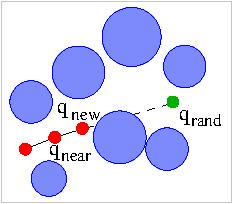
\includegraphics[width=0.25\textwidth]{fig/blosexp2} & 
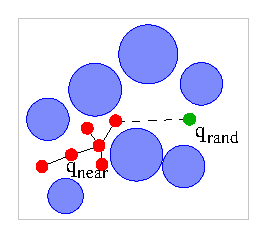
\includegraphics[width=0.25\textwidth]{fig/blosexp3} \\
a & b & c
\end{tabular}
}
\caption{\label{fig::blossom}
    The expansion of the tree using multiple nodes increases the chance to connect the tree with new samples.
For a random sample $\qrand$, its nearest neighbor $\qnear$ in the tree is found (a).
In the straight-line expansion, the tree is expanded by a configuration $\qnew$ located on the line from  $\qnear$ to $\qrand$ in the distance $\varepsilon$ from $\qnear$ (b).
However, the tree cannot be expanded more towards $\qrand$ from $\qnew$ as it is blocked by an obstacle (atom).
By adding multiple nodes around $\qnew$, the tree can be expanded further to $\qrand$ (c).
}
\end{figure}





After a node $\qnear \in \T$ for the expansion is determined, its neighborhood in the distance $\probe$ is sampled using $m$ samples in order to find a configuration $q'$ that is collision-free (at radius $\probe$) and maximally approaches the random configuration $\qrand$.
The resulting configuration $q'$ is added to the tree.
To further expand the tree, the neighborhood of $q'$ is explored again using $n$ new samples.
The samples are generated from the Gaussian distribution with center in $q'$ and $\sigma=\probe$.
A sample $q$ is added to the tree if it is collision-free (i.e., $r(q) \ge \probe$) and if it does not regress the tree.
A sample $q$ is regressing if its nearest neighbor in the tree is closer than $\qnear$.
The regression test prevents the expansion to regions that are already filled densely with other nodes of the tree~\cite{kalisiakBlossom}.
In the first phase of the algorithm, also the distance to the surface atoms is checked.
If the node is too close to the surface, a new blocking sphere is introduced (Alg.~\ref{alg::expand}, line~\ref{alg::expand::bl}).

This expansion by multiple nodes results in dense trees that penetrate the narrow passages more than the classic RRT.
The reason is that if $\qnear$ lies in a narrow passage, the na\"{i}ve straight-line expansion towards the random sample $\qrand$ is more likely prevented by an obstacle located on the line connecting $\qnear$ and $\qrand$.
However, it is still possible that $\qnear$ can be expanded in a different direction, which is realized by the proposed modification.
This increases the chance that $\qnear$ is expanded by at least one new node, which is important especially in the narrow passages.
An example of this is depicted in Fig.~\ref{fig::blossom}.


\begin{algorithm}
{\small
\caption{\label{alg::expand}expandTree($\T, \qnear, \qrand$)}
\KwIn{
    configuration tree $\T$, node for expansion $\qnear$, random sample $\qrand$
}
\KwData{
    probe radius $\probe$, 
    radius to detect exit points $\gprobe$,
    threshold to detect blocking spheres $\dts$,
    number of samples $m$ to generate around $\qnear$,
}
\KwOut{
    expanded tree $\T$,
    list of exit points $P$, 
    blocking spheres $\SB$
}
\hrule
$r_{max} = -1$\; 
$q' = \emptyset$ \;
$d = \infty$\;
$\SB = \emptyset$\;
\For{$i = 1,\ldots,m$}{
    $q$ = random sample around $\qnear$ from $\sim N(\qnear,\probe)$\;
    \If{$r(q) \ge \probe$ {\bf and} $r(q) > r_{max}$ {\bf and } $\dist(q,\qrand) < d $  }{
        $q' = q$\;
        $r_{max} = r(q)$\;
        $d = \dist(q,\qrand)$;
    }
}
$P = \emptyset$; // list of exit points \\
\If{$q' \ne \emptyset$}{
    addNodeToTree($\T,q'$)\;
    addEdgeToTree($\T, (\qnear, q')$)\;
    \For{$i = 1,\ldots,m$}{
        $q$ = random sample around $q'$ from $\sim N(q',\probe)$\;
        $q_n$ = nearestNode($\T, q$)\;
        \If{$r(q) \ge \probe$ {\bf and} $\dist(q,q_n) > \dist(\qnear, q)$}{
            addNodeToTree($\T, q$)\;
            addEdgeToTree($\T, (q',q)$)\;
            $d$ = distance from $q$ to the nearest atom surface $\SSA^i$\; \nllabel{alg::expand::surf}
            \If{$phase=1$ {\bf and } $d < \dts$}{
                $\SB = \SB  \cup \{ \Sgprobe(q) \} $;// $q$ is close to the surface \nllabel{alg::expand::bl}
            }
            \If{$r(q) \ge \gprobe$}{
                $P = P \cup \{q \}$; // new exit point detected \\
            }
        }
    }
}
\return $\T, P, \SB$
}
\end{algorithm}


\section{Detecting Void Space Through the Protein Dynamics}

Detection of dynamic tunnels requires to track the evolution of the void space through the molecular dynamics simulation.
The sequence of protein dynamics is searched by the repeated construction of the collision-free tree and its transfer to the next frame.
The relations between the void space of the previous frame and the void space transferred to the new frame are maintained.
It is necessary to support splitting and merging of the detected void space.
The splitting is caused by atoms that move in the next frame to a part that was detected as void space in the previous frame.
This splitting is achieved during the transfer of the tree to the next frame.
The merging is an inverse process, where a previously unconnected regions of the void space can be connected again.
The splitting and merging are illustrated in Fig.~\ref{fig::merging}.
These two procedures are described in the next subsections.

\begin{figure}
\centering
{
\renewcommand{\tabcolsep}{1pt}
\begin{tabular}{cccccc}
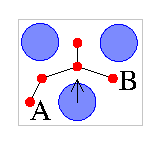
\includegraphics[width=0.15\textwidth]{fig/merging1} &
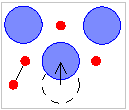
\includegraphics[width=0.15\textwidth]{fig/merging2} &
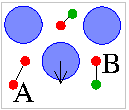
\includegraphics[width=0.15\textwidth]{fig/merging3} &
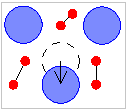
\includegraphics[width=0.15\textwidth]{fig/merging4} &
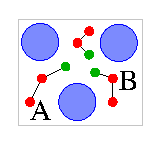
\includegraphics[width=0.15\textwidth]{fig/merging5} &
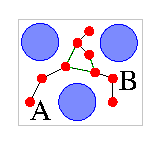
\includegraphics[width=0.15\textwidth]{fig/merging6}  \\
a (frame $i$) & b (frame $i+1$) & c (frame $i+1$) & d (frame $i+2$)  & e (frame $i+2$) & f (frame $i+2)$ \\
detected      & tree transfer   & void space      & tree transfer    & void space      & merging   \\
void space    & (splitting)      & detection       &  (splitting)     &  detection      & \\              
\end{tabular}
\caption{\label{fig::merging}
An example of merging.
The tree in the first frame with a denoted motion of one of the atoms (a). 
A path exists between the nodes $A$ and $B$.
The moving atom in the second frame causes splitting of the detected void space to three components (b).
The components are expanded by new nodes (green) in the frame $i+1$ (c), but they are still too far so merging cannot connect them.
There is not any path between $A$ and $B$ in the frame $i+1$. 
In the third frame, atoms move back without colliding with any of the void space nodes (d).
The three components are further expanded (green nodes) in the third frame (e), but still there is not any path between $A$ and $B$.
The merging in the $i+2$ frame connects the tree components again (dotted lines) (f).
The result of the merging process is again the existing path between $A$ and $B$.
}
}
\end{figure}



\subsection{Tree Transfer}

The transfer of the tree to the next frame of molecular dynamics is listed in Alg.~\ref{alg::transfer}.
The collisions between the nodes of the actual tree and the atoms in the next frame are checked and the colliding nodes are removed.
It is also necessary to remove the nodes outside the protein (these nodes are added in the second phase of the void space detection in order to find exit points).
The nodes that are collision-free at radius $\gprobe$ are therefore removed as well.
Example of the removing of these nodes is depicted in Fig.~\ref{fig::tp2}.

The parents of the surviving nodes are changed to the corresponding nodes from the previous tree.
The remaining nodes, though they are mutually disconnected, are stored again in the tree structure.
As the RRT selects the nodes for the expansion only using their distance to the random samples, the edge information is not necessary for their further expansion.

\begin{algorithm}
{\small
\caption{treeTransfer\label{alg::transfer}}
\KwIn{
    configuration space of the actual frame $\CF^i$,
    configuration tree $\T_{i-1}$ constructed at the frame $i-1$
}
\KwData{probe radius $\probe$, goal radius $\gprobe$}
\KwOut{configuration tree $\T_{i}$ valid for frame $i$}
\hrule
$\SB = \emptyset$; // blocking spheres \\
$\T_{i} = $empty tree\;
\For{$q \in \T_{i-1}$}{
    \If(//is collision-free in the new frame?){$q \in \CF^{i}$}{
        \If{$r(q) \ge \probe$ {\bf and} $r(q) < \gprobe$ }{
            addNodeToTree($\T_{i}, q$)\;
            addEdgeToTree($\T_{i}, (q, \T_{i-1}.q)$)\;
        }
        \If(// $q$ is the exit point){$r(q) \ge \gprobe$}{
            $\SB = \SB \cup \{\Sgprobe(q)\}$\;
    }
    }
}
\return $(\T_{i}, \SB)$\;
}
\end{algorithm}


\begin{figure}
\centering
{
\renewcommand{\tabcolsep}{1pt}
\begin{tabular}{cccc}
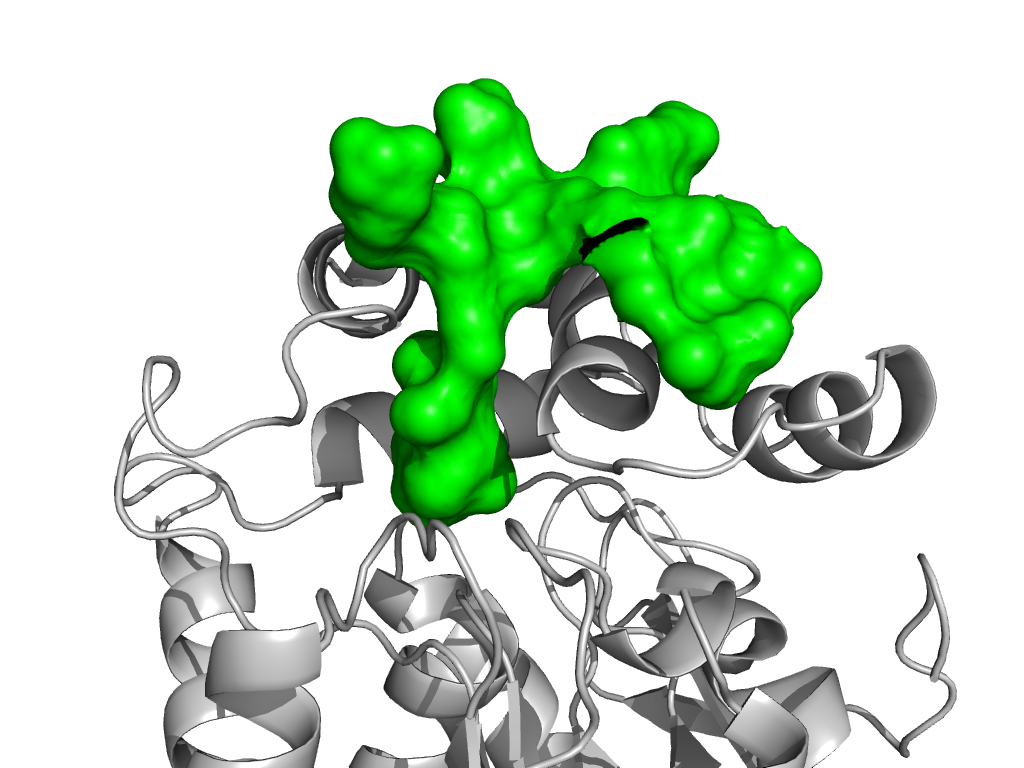
\includegraphics[width=0.24\textwidth]{fig/688a} &
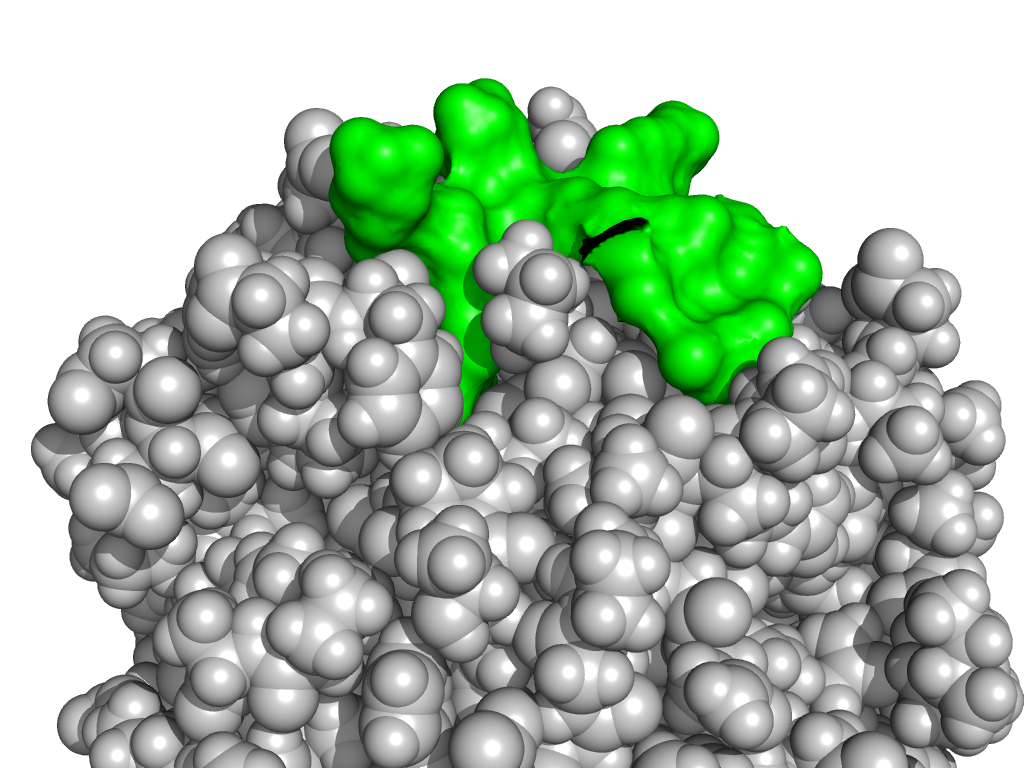
\includegraphics[width=0.24\textwidth]{fig/688b} & 
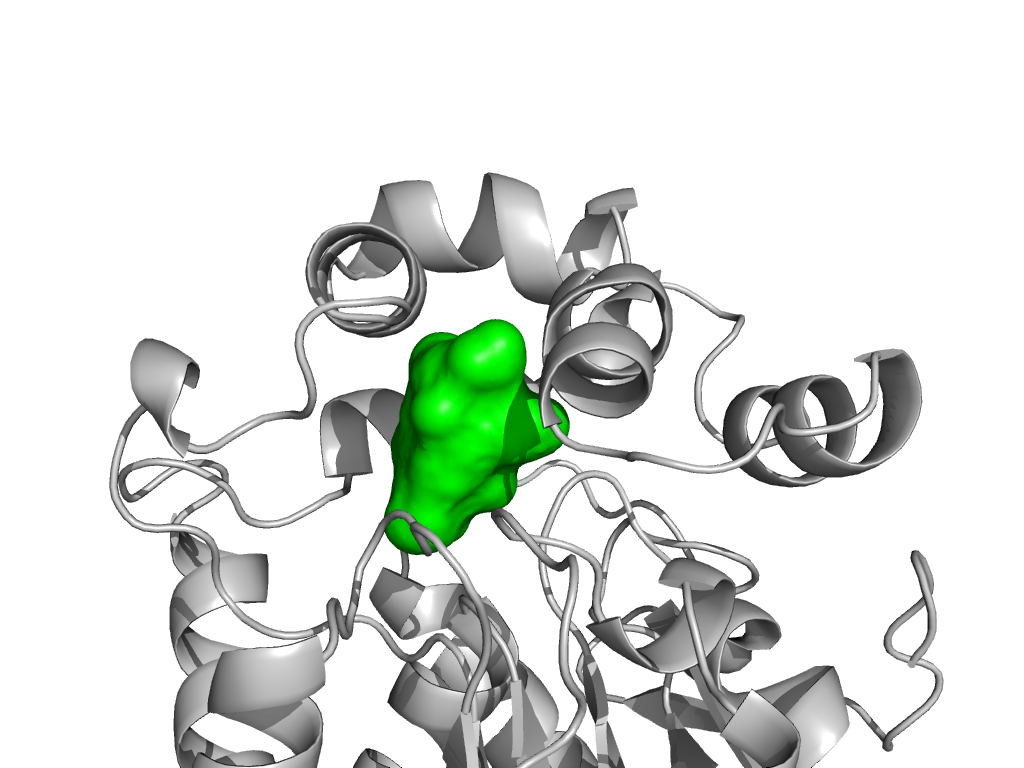
\includegraphics[width=0.24\textwidth]{fig/688d} &
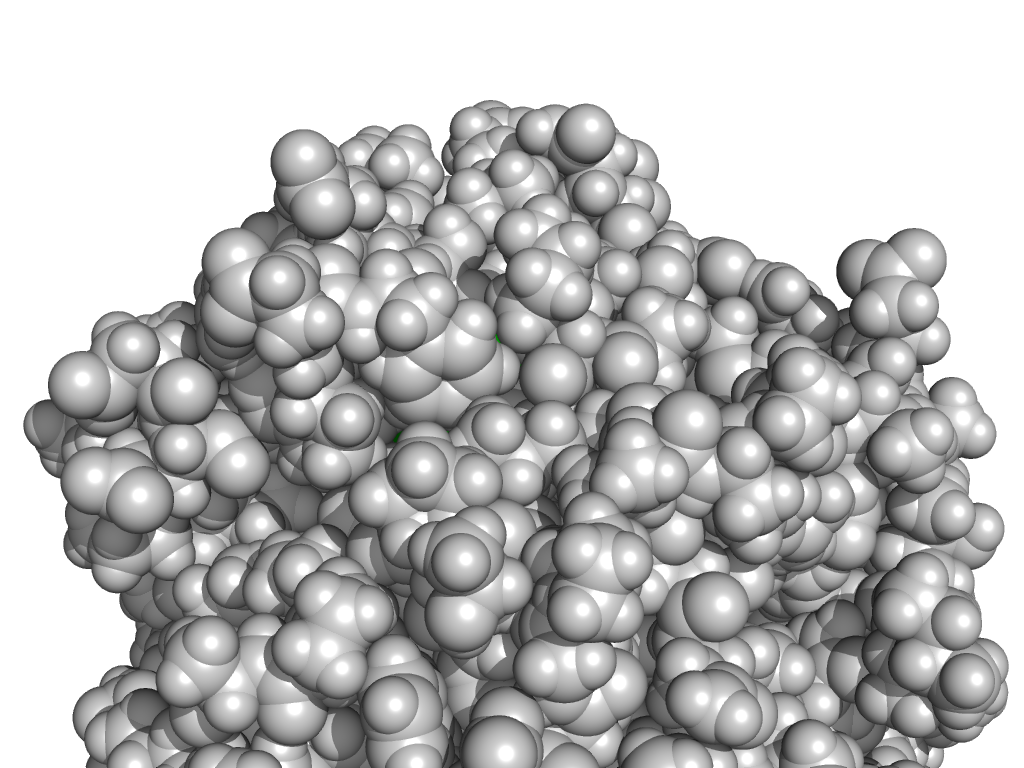
\includegraphics[width=0.24\textwidth]{fig/688c} \\
Frame $i$ & Frame $i$ &  Frame $i+1$ & Frame $i+1$ \\
          & hard-sphere model & & hard-sphere model
\end{tabular}
}
\caption{\label{fig::tp2}
The effect of the tree pruning.
The detected void space is depicted in green.
The void space detected in the frame $i$ is depicted using the cartoon representation as well as the hard-sphere model.
The nodes representing this void space are removed during the pruning phase, as they are collision-free with the radius $\gprobe$.
After the pruning (frame $i+1$), the void space remains only inside the protein (therefore, it is not visible in the hard-sphere
model in the right image).
}
\end{figure}

\subsection{Void Space Merging}

After the tree pruning (Alg.~\ref{alg::transfer}), the parents of the surviving nodes point to the previous frame and the edges connecting the nodes are omitted.
The merging is realized by finding nodes in the tree that can be connected by a collision-free line.
For each node $q$ of the tree, the $k$-nearest neighbors are found and the possibility of their connection is evaluated using collision
detection on the line between them.
The pseudocode of the void-space merging is listed in Alg.~\ref{alg::component}.

The merging results in a graph structure with two types of edges: the edges connecting the nodes within the same frame, and the edges (parent links) connecting some of the nodes with the nodes of the tree from the previous frame.
By computing the components of this graph considering only the first type of edges, we can determine the regions of the void space inside whose the probe can move without any collisions.
The connection of these components to the previous frame is kept in the parent nodes.
This allows us to define a graph $G$ of vod space evolution.
The example of this graph is depicted in Fig.~\ref{fig::transfer}.

\begin{algorithm}
\caption{\label{alg::component}voidSpaceMerging}
{\small
\KwIn{configuration tree $\T$,
}
\KwData{goal-probe radius $\gprobe$,
    probe radius $\probe$, 
}
\KwOut{a set of graph components
}
\hrule

$V$ = vertices of tree $\T$\;
$E = \emptyset$\;
\ForEach{$v \in \T$}{
    $S$ = find $k$-nearest nodes in the tree\;
    \ForEach{$w \in S$}{
        \If{canBeConnected($v,w$)}{
            $d =$ distance from $v$ to $w$\;
            $E = E \cup \{ (v,w,d)\}$; // edge from $v$ to $w$ with weight $d$\\
        }
    }
}
\return $G(V,E)$; 
}
\end{algorithm}




\begin{figure}
\centering
{
\renewcommand{\tabcolsep}{1pt}
\begin{tabular}{cccccc}
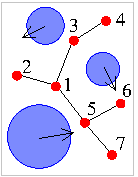
\includegraphics[width=0.19\textwidth]{fig/rrtdyn2} &
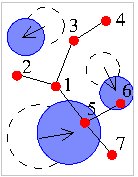
\includegraphics[width=0.19\textwidth]{fig/rrtdyn3} &
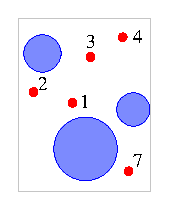
\includegraphics[width=0.19\textwidth]{fig/rrtdyn4} & 
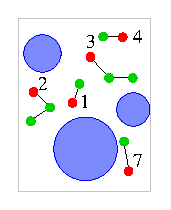
\includegraphics[width=0.19\textwidth]{fig/rrtdyn6} &
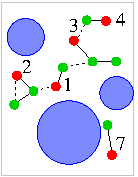
\includegraphics[width=0.19\textwidth]{fig/rrtdyn7} \\
 frame $i$ & frame $i+1$ & frame $i+1$ & frame $i+1$ & frame $i+1$ \\
void space & pruning & after pruning & void space  & merging \\
           &          &                & detection\\
& \multicolumn{3}{c}{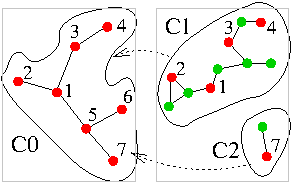
\includegraphics[width=0.4\textwidth]{fig/rrtdyn8}} & 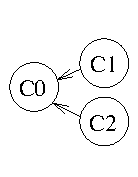
\includegraphics[width=0.19\textwidth]{fig/rrtdyn9} \\
&  \multicolumn{3}{c}{ frame $i$ \hskip 28pt frame $i+1$ } & graph of components
\end{tabular}
}
\caption{\label{fig::transfer}
Tree transfer, merging and graph of relations.
In the frame $i$, the void space consists of one component $C_0$ (nodes 1--7).
After the pruning, the nodes leading to collisions with atoms are removed (nodes $5,6$).
The parents of the remaining nodes are set to the same nodes in the previous frame, e.g., parent of node 3 in frame $i+1$ is the node 3 in the frame $i$.
The tree is then again expanded in the new frame (green nodes).
After merging, two components can be identified ($C_1$ and $C_2$). 
Since some of the nodes of these components point to the previous frame (the red nodes),
      both components $C_1$ and $C_2$ are connected to $C_0$.
}
\end{figure}





\subsection{Tracking the Evolution of Void Space in Molecular Dynamics}

This section presents the main algorithm to track the evolution of the void space in molecular dynamics.
This algorithm relies on all the previously described methods and it is listed in Alg.~\ref{alg::dynamic}.
The search starts with the first frame in the configuration $\qinit \in \CF^1$ that represents the initial position of the active site.
The tree from the previous frame is first transferred to the actual frame and the void space is searched in the given frame using Alg.~\ref{alg::main}.
This results in a new configuration tree and also in a new set of exit points.
After $n$ frames are processed, the algorithm results in $n$ configuration trees.

\begin{algorithm}
%\setstretch{\straa}
{\small
\caption{Tunnel detection in dynamic protein
\label{alg::dynamic}
}
\KwIn{
    starting point $\qinit \in \CF$ in the first frame
}
\KwOut{list of configuration trees $\T_i$\;
}
\hrule
$\T_0$.add($\qinit)$\;
$P = \emptyset$; // list of all exit points \\
$G = $ empty graph\;
\For{$i  = 1 : n$}{
    $(\T_i, \SB)$ = treeTransfer($T_{i-1}, \CF^i$); // Alg.~\ref{alg::transfer}\\
    $(\T_i, P')$ = voidSpaceDetection($\T_{i},\SB)$; //Alg.~\ref{alg::main}\\
    $(V,E) =$ voidSpaceMerging($\T_{i}$); // V,E is a graph of merged void space
    $C$ = find components in the graph (V,E)\;
    add components $C$ to graph $G$
    connect exit points $P'$ with their components in $G$\;
    connect active site $\qinit^i$ with its component in $G$\;
}
}
\end{algorithm}



\subsection{Reconstruction of the Static and Dynamic Tunnels}

After the void space is detected in all frames by Alg.~\ref{alg::dynamic}, the tunnels can be identified using the graph $G$ describing the evolution of the void space.
The nodes in this graph are the components of the void space in each frame, the directed edges connect the components from the frame $i$ with the previous frame $i-1$ and the undirected edges connect the exit points and the active sites to their components.

One tunnel is defined by an exit point and by an active site.
If both these nodes are connected to the same component of the graph, they define a static tunnel.
Such a tunnel can be reconstructed simply by finding a path between these two nodes in the graph.
If there does not exist any path between the exit point $p \in P^i$ (exit point at frame $i$) and the active site $\qinit^i$ in the same frame, the dynamic tunnel has to start from a different active site (in one of the previous frames).
A path from $p$ to the first active site reachable in the graph (measured by the number of edges) describes the dynamic tunnel.
An example is depicted in Fig.~\ref{fig::components}.

There are two possible reasons why the active site of the same frame cannot be reached.
First, the exit point is not connected with the same component of the graph as the active site.
Second, the active site does not exist in the given frame, which may happen if large probes are considered.

\begin{figure}
\centering
{
\renewcommand{\tabcolsep}{0pt}
\begin{tabular}{cccc}
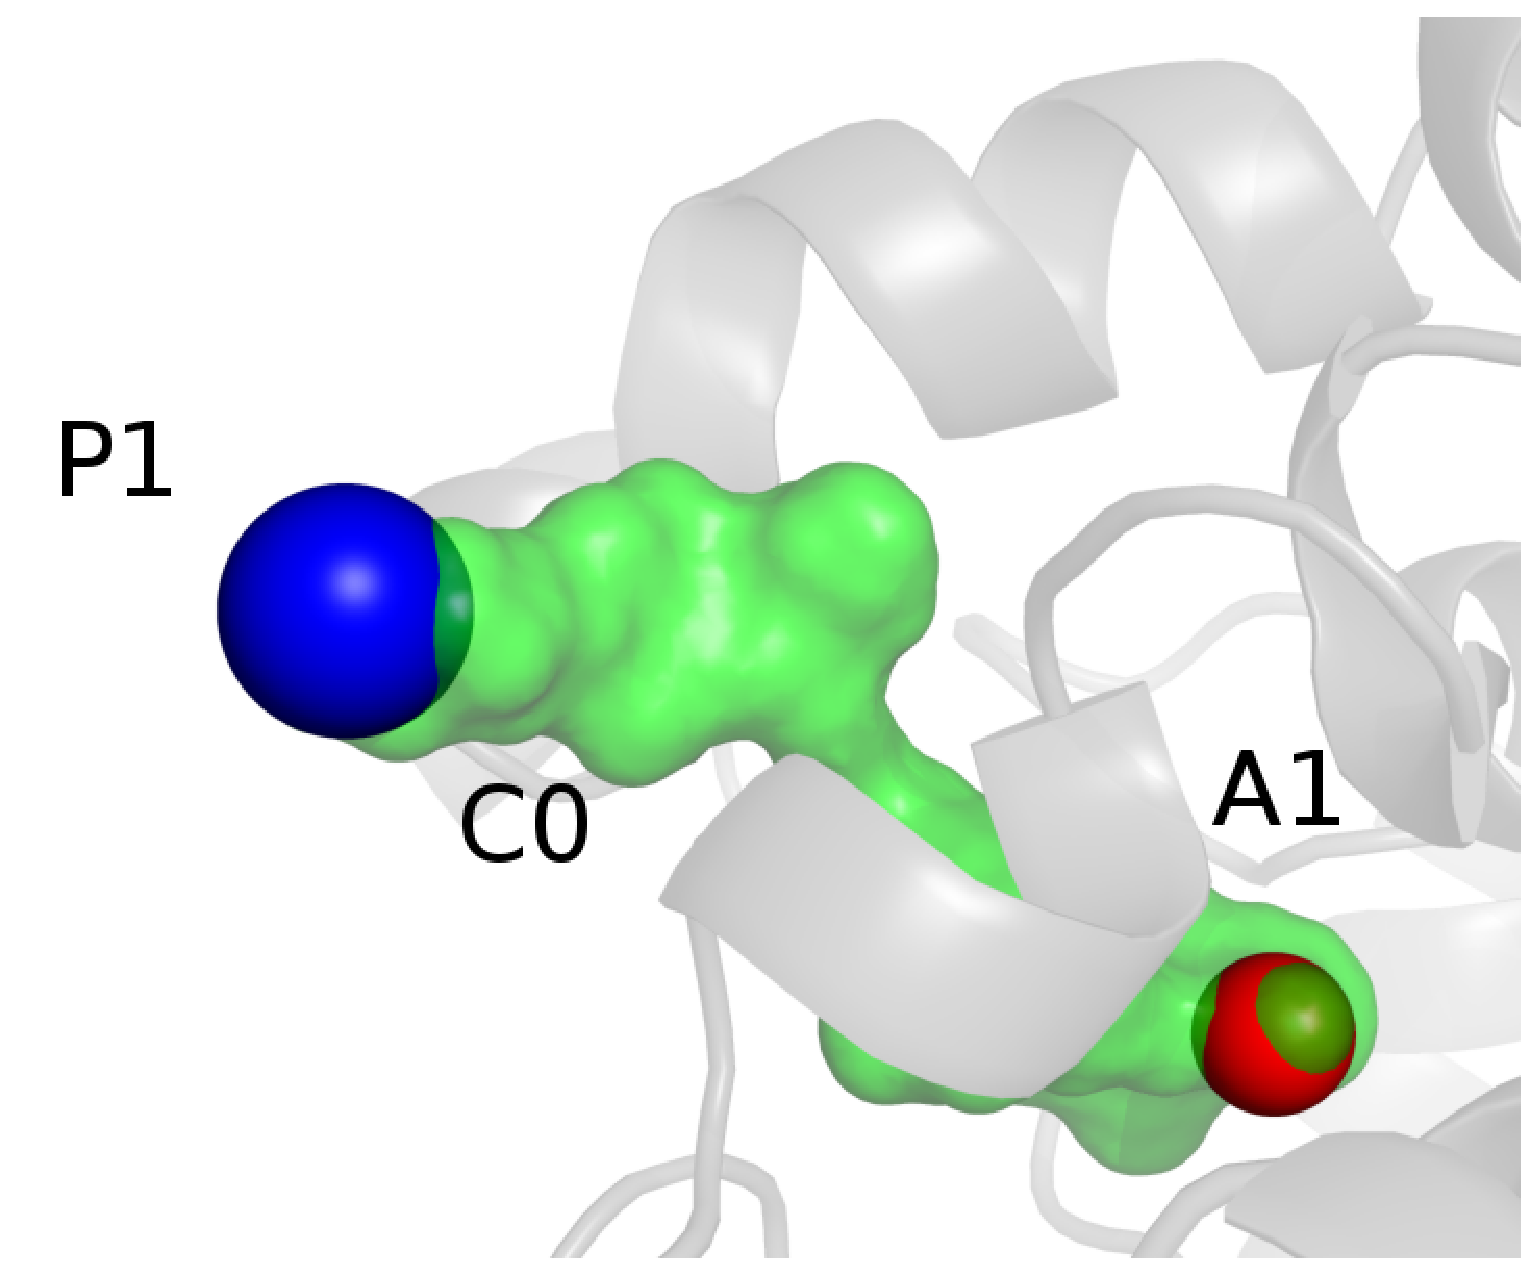
\includegraphics[width=0.24\textwidth]{fig/com1label} & 
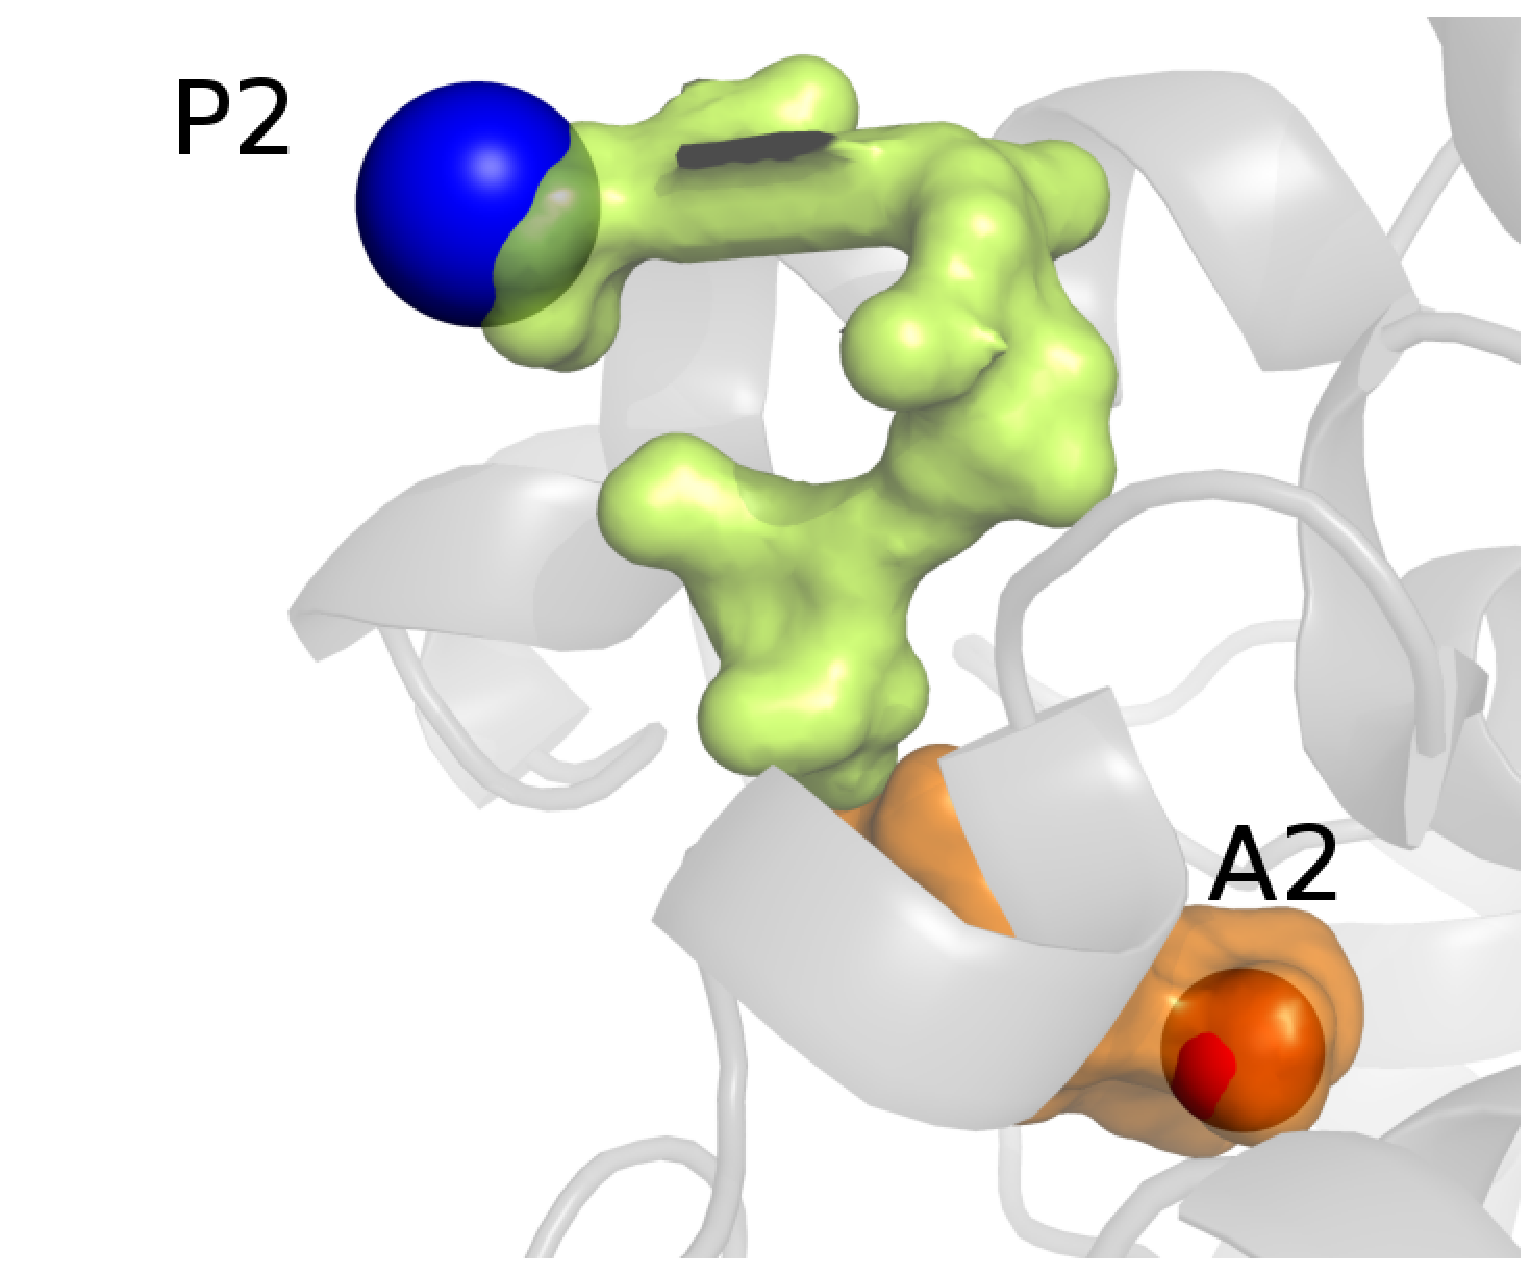
\includegraphics[width=0.24\textwidth]{fig/com8label} &
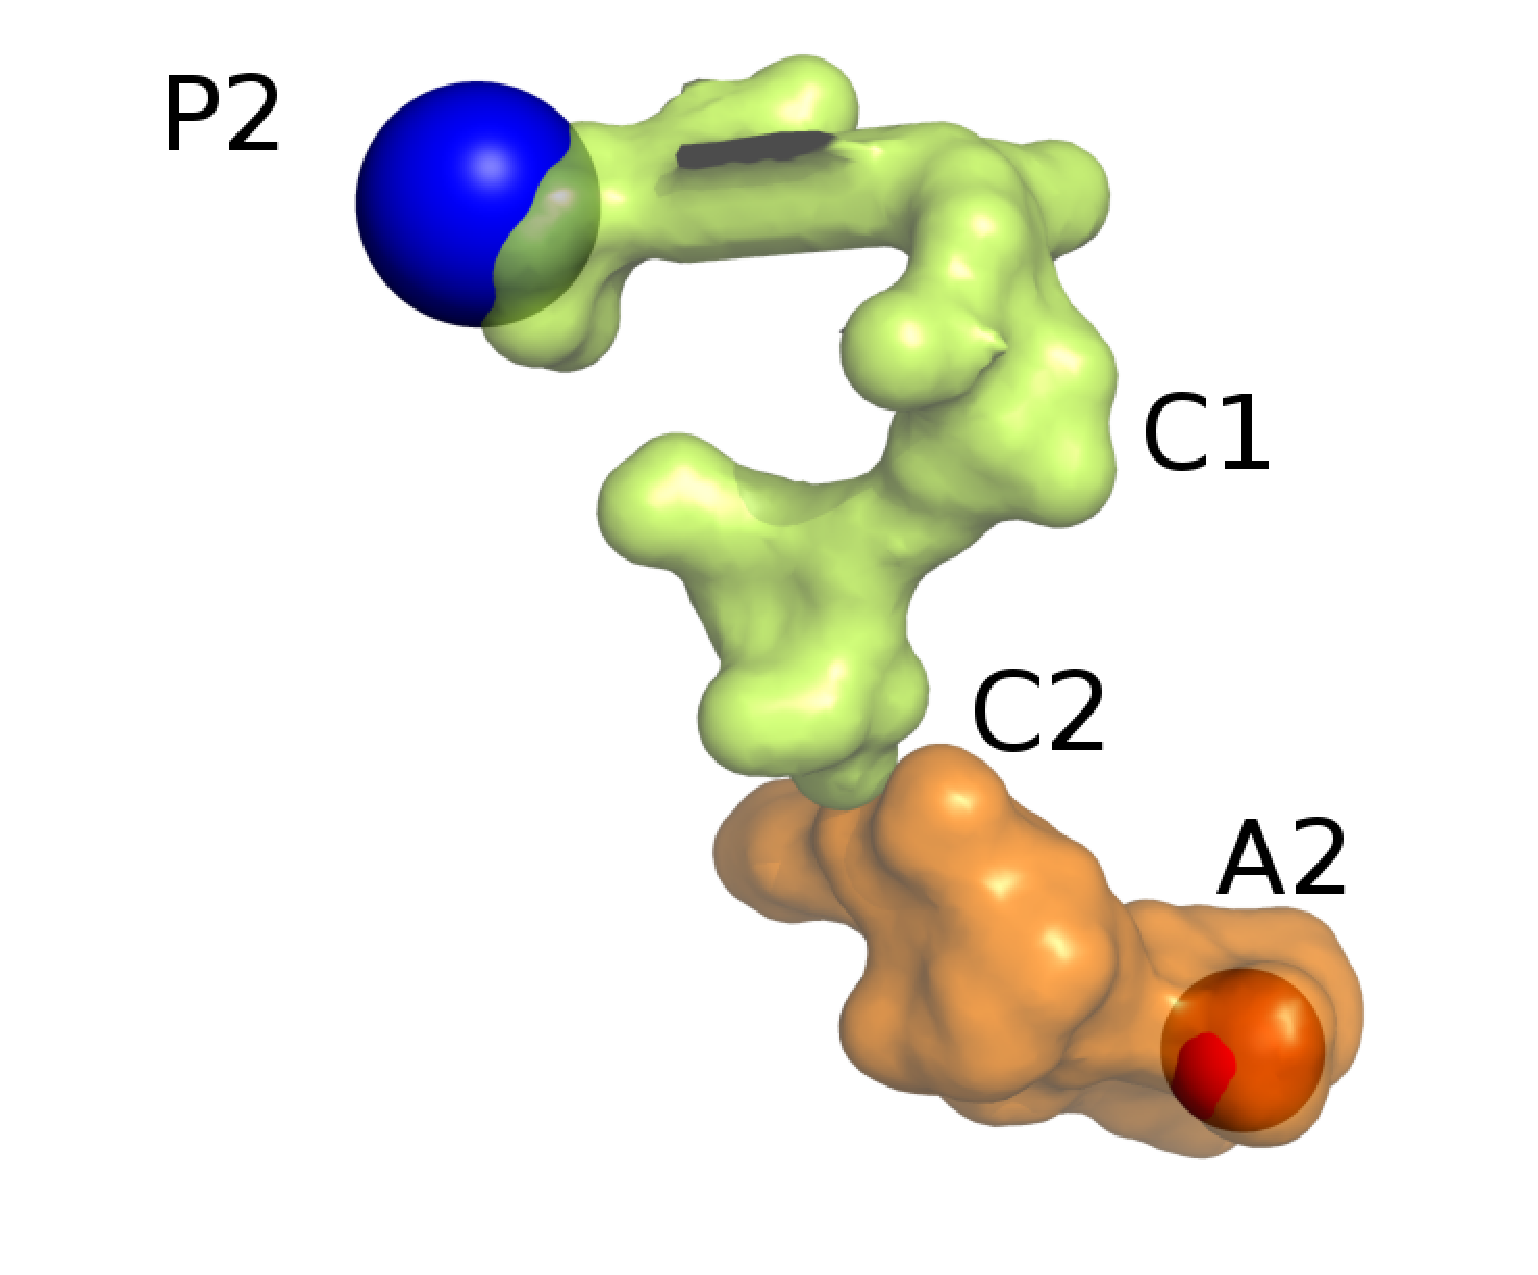
\includegraphics[width=0.24\textwidth]{fig/com7label} & 
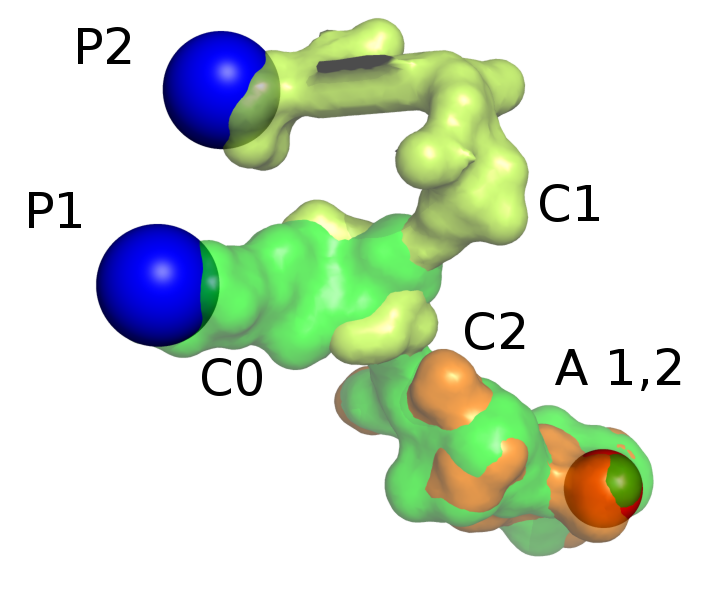
\includegraphics[width=0.24\textwidth]{fig/com12label} \\
a (frame $i$) & b (frame $i+1$) & c (frame $i+1$) & d (frame $i$ and $i+1$) \\
\multicolumn{4}{c}{
    \includegraphics[width=0.3\textwidth]{fig/comp1}\hskip 5pt
    \includegraphics[width=0.3\textwidth]{fig/comp2} \hskip 5pt
    \includegraphics[width=0.3\textwidth]{fig/comp3}
}\\
\multicolumn{4}{c}{%
    \hskip 5pt e (connections in frame $i$) 
    \hskip 5pt f (connections in frame $i+1$) 
    \hskip 5pt g (connections from $i$ to $i+1$) 
}
\end{tabular}
}
\caption{\label{fig::components}
An example of components in two consecutive frames found in an MD simulation of the 1CQW protein.
The void space (green) is detected in the frame $i$ and both the exit point ($P_1$) and the active site ($A_1$) are connected with the same component $C_0$ (green).
A static tunnel can be found between the active site and the exit point $P_1$ (a).
In the second frame, the void space splits to two components $C_1$ and $C_2$ (yellow, orange) (b,c).
The exit point $P_2$ is connected to $C_1$, while the active site is connected to $C_2$.
There is not static tunnel between $P_2$ and $A_2$, as the components $C_1$ and $C_2$ are not connected.
Hence, $P_2$ indicates the end of a dynamic tunnel.
This tunnel is reconstructed by finding a path from $P_2$ to any closest reachable active site in the previous frame.
In this case, the dynamic tunnel is described by the path $P_2, C_1, C_0, A_1$. 
This dynamic tunnel evolves from $A_1$ of frame $i$ to exit point $P_2$ in the frame $i+1$.
}
\end{figure}



\subsection{Implementation Details}

The proposed algorithm relies on two main techniques: the collision detection and the nearest-neighbor search.
Fast collision detection can be generally realized using hierarchical data structures like AABB or OBB trees~\cite{ericsonRTCD}.
The BioCD collision detection is ~\cite{angulo2005biocd} is dedicated for protein structures.
The nearest-neighbor search can be realized fast using KD-trees. 
The new nodes added to the configuration tree has to be also added to the KD-tree structure, so the KD-tree should support
fast insert operation. 
MPNN~\cite{yershovaMPNN} was designed for the purpose of sampling-based motion planning and it is used also in our implementation.

The void space detection depends on several parameters like the number of iterations $\Imax$, the number of
samples in the expansion step $m$, and the parameters $\da$ and $\db$ controlling the selection of active Voronoi vertices.
Increasing $\Imax$ and $m$ generally allows us to construct larger configuration trees.
The growth of the tree inside the proteins is limited not only by the atoms, but also by the blocking spheres.
Moreover, the regression test performed before adding a new sample to the tree ensures that the tree does not grow towards its own nodes.
If the tree already fills the void space, the expansion will not add new nodes and therefore, using too high values of $\Imax$ 
does not make sense.

Protein structures vary in the number of atoms, roughness of their surface, size of the internal cavities etc. 
Therefore, there is no universal setting of these parameters and they have to be adjusted considering a given protein.
This is similar to the preparation of VD-based tunnel detection, where several parameters  also have to be specified for the given protein.
The authors' best practices is to test several setting of the parameters and judge them using visual inspection on several frames.
The number of iterations $\Imax$ has to allow the tree to fill the internal void space and (in combination with the length of the second phase of the method), it should allow to detect the exit points.
A simple test to find a good $\Imax$ is to increase it incrementally, detect static tunnels in a single frame and count the number of unique tunnels.
After a certain value of $\Imax$, the number of unique tunnels does not increase and it does not make sense to use higher value.


In comparison to classic RRT, which adds only one node to the tree per iteration, the proposed method can expand the tree by up to $m+1$ nodes.
Consequently, the number of collision detection queries is $m$ times higher in each iteration.
The nearest-neighbor search is used more times, than in classic RRT, because  the nearest-neighbor search is used to update the active Voronoi vertices.
The complexity of the update of the active Voronoi vertices is $\mathcal{O}(|\VV^i|\log(|\T|))$, where $|\T|$ is the number of nodes in the tree, assuming that the nearest neighbor search is realized using KD-trees.
For the sake of simplicity, we update $\VVA^i$ in each step in the pseudocode (Alg.~\ref{alg::main}), but practically, it is not necessary.
The tree expands incrementally, and usually it takes many iterations before most of the active Voronoi vertices are reached by the tree.
It is therefore possible to update these vertices, e.g., in every $n$-th iteration. 

The other usage of nearest neighbor-search is to compute the distance to surface atoms (Alg.~\ref{alg::expand}, line~\ref{alg::expand::surf}).
The complexity of this step is $\mathcal{O}(\log( |\SSA|)$, where $|\SSA|$ is the number of the surface atoms.
The number of the surface atoms depends on the number of atoms in the protein as well as the radius $\gprobe$, that is used to detect the surface atoms.
For a protein with $\sim 5000$ atoms and $\gprobe=4$~\AA, the number of surface atoms is $\sim800$, and therefore the checking
of proximity to surface atoms using KD-trees is negligible. 
An example of the surface atoms is depicted in Fig.~\ref{fig::surface}.

Each frame can be processed separately and it is not necessary to hold all the data structures from all previous frames in memory.
This is valid for all data structures like nearest-neighbor search, collision detection and the configuration tree.
The only exception is the tree pruning (Alg.~\ref{alg::transfer}), where both the tree from the previous frame and the new tree has to be stored in the memory.
After the tree is transferred to the next frame, the old tree does not need to be stored in the memory.
The reconstruction of the tunnels requires to search graph of the components. 
As each frame results in few (or maximally tens) of components, hence searching this graph also does not have high memory requirements.


\begin{figure}
\centering
\begin{tabular}{cc}
\includegraphics[width=0.3\textwidth]{fig/1mxta-alpha4} &
\includegraphics[width=0.3\textwidth]{fig/1mxta-alpha3} \\
a & b
\end{tabular}
\caption{\label{fig::surface}
Example of the surface atoms on the protein PDB ID 1MXT. The hard-sphere model colored by atom type (a), the surface atoms are highlighted in brown (b).
}
\end{figure}


\section{Experimental Verification}

Our proposed algorithm has been tested on several MD simulations obtained by the domain experts. 
Here we present the results of one such a study, performed on an MD consisting of 8,000 frames of the DhaA haloalkane dehalogenase protein (PDB ID 1CQW).
The molecular dynamics was simulated using the AMBER tool.
The active site was defined by the surrounding residues with sequence numbers 38 (Asparagine), 102 (Histidine), and 103 (Aspartic Acid).
The tunnels were investigated for $\probe=1.4$~\AA.


First, in each frame the static tunnels were detected using the CAVER 3.0~\cite{caver3} state-of-the-art tool.
The exits of these tunnels were defined using solvent radius 4~\AA.
In 2,860 frames, the CAVER tool did not detect any static tunnel, 5,100 frames contained only one tunnel, and in 40 frames CAVER found even two tunnels.

The same dataset has been scrutinized by our proposed algorithm for detection of dynamic tunnels.
The positions of the active site in each frame were taken from the results of the static tunnel detection (from those frames, where at least
one static tunnel was detected).
%(i.e., the position of the active site was not known for 2860 frames).
The goal region of the protein was defined in the same way as for the static tunnel detection, i.e., $\gprobe=4$~\AA\ and 
the surface atoms were detected using the $\alpha$-shape with the same radius.

In each frame, the void space detection (Alg.~\ref{alg::main}) was performed with $\Imax=1200$ iterations.
The second phase of the search was switched after $\alpha=70$~\% of the iterations (i.e., after 840 iterations).
Other parameters and their values used for the computation were $m=8$, $\da=5$~\AA, $\db=0.5$~\AA, $\gb=0.1$, and $\dts=2$~\AA.

In each iteration, up to $m=8$ new samples can be added to the tree which can result in up to $1,200 \times 8 = 9,600$ new nodes in each frame. 
The number of the tree nodes does not rise during the computation because many of the nodes are pruned.
The average tree size is 3,924 (std.dev 1,154) nodes.
The size of the built tree together with the number of detected components in each frame are depicted in Fig.~\ref{fig::treesize}.
The example of the detected void space is depicted in Fig.~\ref{fig::dyn}.

\begin{figure}
\centering
{
\renewcommand{\tabcolsep}{0pt}
\begin{tabular}{cc}
\includegraphics[width=0.48\textwidth]{fig/probe14treeSize} &
\includegraphics[width=0.48\textwidth]{fig/probe14components}  \\
a & b  \\
\end{tabular}
}
\caption{\label{fig::treesize}
    The number of nodes in the tree representing the void space (a) and the number of graph components in each frame
        of molecular dynamics simulation (b).
}
\end{figure}


\begin{figure*}
\centering
{
\def\ee{0.26}
\renewcommand{\tabcolsep}{-1pt}
\begin{tabular}{cccc}
\includegraphics[width=\ee\textwidth]{fig/video-0560} &
\includegraphics[width=\ee\textwidth]{fig/video-0561} &
\includegraphics[width=\ee\textwidth]{fig/video-0562} &
\includegraphics[width=\ee\textwidth]{fig/video-0563}  \\
Frame 560 & Frame 561 & Frame 562 & Frame 563 \\                       
\includegraphics[width=\ee\textwidth]{fig/video-0699} &
\includegraphics[width=\ee\textwidth]{fig/video-0700} &
\includegraphics[width=\ee\textwidth]{fig/video-0701} &
\includegraphics[width=\ee\textwidth]{fig/video-0702}  \\
Frame 699 & Frame 700 & Frame 701 & Frame 702   \\                       
\end{tabular}
}
\caption{\label{fig::dyn}
Evolution of the void space in molecular dynamics of the DhaA protein. 
In frames 560--563, the active site is contained in the detected void space (red sphere).
On the contrary, the void space (for probe 1.4~\AA) detected in frames 699--701 does not contain the active site.
The active site appears again inside the void space in frame 702.
}
\end{figure*}


\begin{table}
\centering
\caption{\label{tab::dyn} The number of frames with detected dynamic tunnels. The number of frames
    with static tunnels, detected by CAVER 3.0.
}
\begin{tabular}{ccccc}
\toprule
  \multirow{2}{*}{ Dynamic tunnel}   &  \multicolumn{2}{c}{ Static tunnels}   \\
                                     &  {\bf Exists} & {\bf Not exists} \\
\midrule                                     
{\bf End of tunnel/cavity}           & 1,324/661 & 1,027/725  \\
{\bf Static tunnel}                  & 3,118     &  0   \\
{\bf No tunnel}                      & 669      & 1,833    \\ 
\bottomrule                                 
\end{tabular}
\end{table}

The number of frames where dynamic tunnels were detected is summarized in Tab.~\ref{tab::dyn}.
In 2,860 frames, no static tunnel was found by CAVER, but  in 1,027 of these cases, a dynamic tunnel was detected and
in other 725 frames, a part of the tunnel (cavity) was detected.
The total number of frames where either end of dynamic tunnel was detected or a cavity that is part of a dynamic tunnel was
1,197.
This shows that the proposed dynamic tunnel detection can bring new information about 1,197 of tunnels, that would be 
discarded in the analysis based solely on static tunnels.
No static tunnel was identified by the proposed method in frames, where no frames were detected by CAVER.
This is not surprising, as there are no active site in these frames so neither static or dynamic tunnel can start in them.
No dynamic neither static tunnel was identified in 1,833 frames and therefore, behavior in these frames  remains unknown.
The results also show that no static tunnel was identified in 669 frames by the proposed method, while CAVER detected static tunnels there.
%The number of frames where the dynamic tunnels were detected is summarized in Tab.~\ref{tab::dyn}.
%In 2,860 frames, no static tunnel was found by CAVER, but in 1,027 frames of this set, a dynamic tunnel was detected.
%Both static and dynamic tunnels were detected in 1,324 frames.
%These results bring new information about the protein behavior. 
%They show that a path connecting the protein surface with the active site is more frequent than the static tunnels suggest.
%The examples of frames without a static tunnel, but containing a dynamic one, are depicted in Fig.~\ref{fig::seq1}.
%
%
%In the case of 3,816 frames where a static tunnel was detected by CAVER, no dynamic tunnel was detected by the proposed method. 
%3,118 frames out of 3,816 were identified as static.
%This indicates that some tunnels were detected as dynamic instead of static.
The proposed method is non-deterministic and it may happen, that some part of the tree does not reach the outer region of the protein and consequently, some exit points are not detected, which decreases the numbef detected static tunnels.
These missed exit points are then reached in the next frame which leads to the detection of the dynamic tunnel.
The number of correctly classified static tunnels can be increased by using higher $\Imax$.
In our experiment, $\Imax=1,200$ was used with a lower value in order to process the whole sequence of 8,000 frames in a reasonable time.

The computation was realized on Intel(R) Xeon(R) CPU E5-2630 v2 @ 2.60GHz with 64GB of RAM using one thread.
As the algorithm holds in the memory only the actual tree (which has less than 10,000 nodes in most of the cases),
the maximally allocated memory during the computation was less than 1GB.
The average computation time to process one frame is 15~s.
In comparison, the computation of the static tunnels using CAVER 3.0 tool takes $\sim$11s per frame.
The processing times for a long sequence of 8,000 frames leads to around 33 hours of computation on a single processor.
Such time is still negligible in the comparison to the preparation of the molecular dynamics simulation.
%Times: 8000 frames, cca 35 hodin = cca 15s/frame. Caver na mem ntb: cca 11s/frame.

The examples of frames without a static tunnel, but with a dynamic one, are depicted in Fig.~\ref{fig::seq1}.
A static tunnel and also a dynamic tunnel was detected in 1324 frames.
These results bring new information about the protein, as they show, that a pathway to the active site exists more
frequently than is described by the classic static tunnels.



Many dynamic tunnels were discovered in the studied protein dynamics.
The inspection of the detected tunnels utilizes a simple visualization which shows all parts of the dynamic tunnel in one frame.
The example of this type of visualization is depicted in Fig.~\ref{fig::joint}.
Such visualization allows the biochemists to identify the surrounding residues and further study their physico-chemical properties and their influence on the tunnels.
For the analysis of a large simulation, an aggregation of the results is necessary.
In~\cite{fig::vis1}, the dynamic tunnels are visualized using vertical bars colored according to the number of frames occupied by this tunnel.


   
    
\begin{figure}
\centering
\includegraphics[width=0.33\textwidth]{fig/58-60crop}
\includegraphics[width=0.33\textwidth]{fig/280-283crop}
\includegraphics[width=0.28\textwidth]{fig/263-267crop}
\caption{\label{fig::joint}
Examples of visualization of the dynamic tunnels evolving over three, four, and five frames. Different colors depict different frames of the dynamic tunnel. This enables the users to easily determine the portion (length) of the tunnel which was detected in the corresponding frame. 
}
\end{figure}


\begin{figure*}
\centering
{
\renewcommand{\tabcolsep}{0pt}
\begin{tabular}{cccc}
\includegraphics[width=0.24\textwidth]{fig/framed-0033-001-0032} & 
\includegraphics[width=0.24\textwidth]{fig/framed-0033-002-0033label} &
\includegraphics[width=0.24\textwidth]{fig/framed-0033-002-0032} & 
\includegraphics[width=0.24\textwidth]{fig/framed-0033-001-0033label} \\
\multicolumn{2}{c}{tunnel I, frames 32-33} &
\multicolumn{2}{c}{tunnel II, frames 32-33} \\
\includegraphics[width=0.24\textwidth]{fig/framed-0053-000-0049} &
\includegraphics[width=0.24\textwidth]{fig/framed-0053-000-0050} &
\includegraphics[width=0.24\textwidth]{fig/framed-0053-000-0051} &
\includegraphics[width=0.24\textwidth]{fig/framed-0053-000-0053} \\
\multicolumn{4}{c}{tunnel I, frames 49--52} \\
\end{tabular}
\caption{\label{fig::seq1}
Examples of dynamic tunnels.
Two dynamic tunnels were detected in frames 32-33, both ended in different exit points (P1 and P2).
The bottom sequence shows the evolution of a dynamic tunnel over four frames.
The active site (red sphere) is not inside the detected void space in frames 33, 50, and 52, which indicates that any static tunnels
were detected in these frames.
}
}
\end{figure*}



\begin{figure*}
\centering
%\includegraphics[width=0.99\textwidth]{fig/dyn_tunnels_7985}
\includegraphics[width=0.99\textwidth]{fig/5}
\caption{\label{fig::vis1}
Visualization showing the results of the dynamic tunnel detection performed on the MD simulation containing 8,000 frames. 
  Each line corresponds to one detected dynamic tunnel.
  The length of the line depicts the actual length of the tunnel (its centerline). 
  The color corresponds to the number of consecutive frames in whose the given dynamic tunnel was detected (i.e., within these frames the tunnel was able to connect the protein surface with its active site).
    It is clearly visible that most of the dynamic tunnels were constructed within two or three frames. However, there are several tunnels spanning through more frames (up to 35).
}
\end{figure*}


{\textcolor{red}{TODO Fig.~\ref{fig::caver34}.}}

\begin{figure}
\centering
\includegraphics[width=0.9\textwidth]{fig/caver3450-3700_colored}
\caption{\label{fig::caver34}
Visualization of tunnels detected using our method (RRT) in comparison to tunnels detected by CAVER.
Both static tunnels detected by CAVER and by our method are depicted in gray.
Then, colored bars show snapshots where a dynamic tunnel was detected by our algorithm.
The dynamic tunnel bars are colored according to the order in which a snapshot occurs in the dynamic tunnel.
It is visible that our method is able to extract many additional information about the void space than traditional static tunnels computed by CAVER.
}
\end{figure}




\section{Discussion}

The static tunnels computed by the CAVER tool were discovered in 5,140 frames leaving the rest of 2,860 (i.e., 35~\%) 
frames without any further analysis.
Our proposed method was able to further detect dynamic tunnels in other 1,027 frames.


The number of static tunnels decreases with the increasing probe size. 
In order to increase the number of frames with detected static tunnels, the biochemists usually analyze the tunnel with a smaller probe size, e.g., 1~\AA or even 0.9~\AA.
This leads to the detection of more tunnels, but on the other hand, their bottleneck may be too narrow for the passage of certain ligands.
In the described experiment, we analyzed the proteins with a very large probe size (1.4~\AA).

The void space detection is based on the principle of RRT which makes the tunnel detection non-deterministic.
This brings two effects. The static tunnels can be incorrectly classified as dynamic tunnels, and the length/position/bottleneck of the reported tunnels may vary between various runs.
The cause of the former case is that the growth of the tree is blocked, which slows down the reaching of the outer space and consequently any exit points are detected.
To minimize this effect, the dynamic tunnel should be detected primarily on those frames, where any static tunnel does not exist.

Despite this, the second effect remains and the properties of the discovered tunnels may still vary.
The detection should be computed multiple times, evaluating the similarity of the tunnels and reporting more statistically robust results.
A possible solution is either to remove the dependency on the random numbers, e.g., by sampling the void space using Hammersley or Halton sequences~\cite{Lav06,branickyQuasi,rosell2007general}.
However, these extensions are beyond the scope of this paper and they are planned in our future work.



%A possible approach is to generate the random numbers using a deterministic sequence
%\cite{rosell2007general}

%To improve the conectivity of the space, works from the domain of probabilsitic roadmaps can be used.
%\cite{rantanen2011connectivity}






\section{Conclusion }

Tunnels in protein structures connect the active site with the surface of the protein.
The properties of the tunnels like their length or bottleneck radius help chemist to analyze behavior of the proteins.
The classic approach to detect the tunnels is based on finding path in Voronoi diagrams of the protein, which can principally
lead to discovery of only static tunnels, i.e., tunnels that fully connect the active site and the protein surface in one frame.

In this paper we presented the concept of so called dynamic tunnels in molecular dynamics simulations and our proposed algorithm for their detection.
The proposed solution enables the biochemists to detect and trace the void space (i.e., dynamic tunnels) also in those snapshots of molecular dynamics simulations, where the traditional approaches fail.
Additionally, we presented a set of visual representations designed specifically to explore and understand the resulting set of dynamic tunnels detected by our algorithm. 
These representations form an integral part of our solution, namely because of the size and complexity of the results. 
We believe that our solution represents a significant step towards the full tracking of the evolution of the void space inside proteins which can be potentially used for transportation of ligands from the outer environment to the protein active site.




\section{Acknowledgments}

The presented work has been supported by the Czech Science Foundation (GA{\v C}R) under research project No. 17-07690S.
Access to computing and storage facilities owned by parties and projects contributing to the National Grid Infrastructure MetaCentrum, provided under the programme "Projects of Large Infrastructure for Research, Development, and Innovations" (LM2010005), is greatly appreciated.


\bibliographystyle{plain}
\bibliography{paper}

\end{document}


% =======================================================================================
% =======================================================================================
% =======================================================================================
% =======================================================================================
% =======================================================================================
% =======================================================================================
% =======================================================================================

%~\cite{amatoOBPRM,hollemanMAPRM} shift random samples towards medial axis of the environment, which helps to sample
%narrow passages more densely. 
%For example, the random samples generated in the configuration space can be shifted
%towards the medial axis of the environment~\cite{amatoOBPRM,hollemanMAPRM} or even generated around the medial 
%axis~\cite{wilmarthMAPRM,foskey01hybrid,guibas1999probabilistic,hoff2000interactive,yang2004adapting}.
%The paper~\cite{amatoOBPRM} suggests to sample uniformly in the configuration space and shift the samples towards the medial axis.
%Another approach is to generate the samples randomly in \CS\ and shift them closer to the medial axis~\cite{amatoOBPRM}.
%The medial axis can be computed exactly using GVD.
%While the medial axis can be easily computed for 2D or 3D workspaces using GVD, its computation become complicated in many dimensions.
%In such case, the samples can be generated uniformly from the whole \CS\ and moved in an estimated direction towards the medial axis~\cite{hollemanMAPRM}.
%sampling-based for 
%protein-ligand access and docking \cite{bayazit2001ligand,singhLig,apaydin2004stochastic,cortes2010simulating}
%protein and RNA folding~\cite{amatoPF1,ApaBru03}
%protein loop motions~\cite{cortes2004geometric},
%domain motions~\cite{kirillova2008an}, 
%and motions of pairs of alpha-helices in transmembrane proteins~\cite{enosh2007prediction}

%The behavior of RRT in the narrow passages was analyzed using Voronoi diagrams in~\cite{yershovaDDRRT}.
%The nodes in the tree can be divided into two groups: frontier nodes, whose Voronoi cells grow together with growth
%of the environment and boundary nodes, which are close to the obstacles. %~\cite{yershovaDDRRT}.
%The tree cannot be expanded from the boundary nodes.
%In a narrow passage, the nodes are both boundary and frontier.
%These nodes are frequently selected for the expansion, because they are the frontier nodes, however the tree cannot be expanded
%from them, because they are also the boundary nodes. 
%To suppress selection of the boundary nodes, authors of~\cite{yershovaDDRRT} suggest to define an action radius around each node.
%The node is selected for the expansion only if its radius is larger than the distance to the random sample.
%The radius of new nodes is set to $\infty$ and it is decreased to a predefined value $\rdd$ if the node cannot be expanded.
%A Dynamic-Domain strategy for RRT (RRT--DD) is proposed in~\cite{yershovaDDRRT}:
%each node holds an action radius defining how far can be a random sample $\qrand$ that activates the node for the expansion.
%The RRT--DD algorithm generates random samples $\qrand$  and finds its nearest neighbor in the tree
%$\qnear$ until $\rho(\qrand,\qnear) < \qnear.radius$. 
%Although the algorithm is efficient in the narrow passages, it is strongly influenced by the parameter $\rdd$.
%To decrease the sensitivity of the method to the parameter $\rdd$, it can be automatically adjusted, which
%was proposed in RRT--ADD (RRT with Adaptive Dynamic Domain)~\cite{jailletATDDRRT}.
%Another schema to automatically adjust parameters of the RRT-based planners was proposed in~\cite{schneider2015completely}.

%Retraction-RRT~\cite{zhangRetraction} generates random samples uniformly as in the original RRT, but it
%attempts to shift them into the narrow passages.
%A~random configuration $\qrand \in \CF$ is generated and a close non-free configuration $q \in \CO$ is found. 
%A~contact configuration $q_c$ on a segment $(\qrand,q)$ is found and its neighborhood is searched for
%$q_c'$ minimizing the distance between $q$ and $q_c'$. 
%The configuration $q_c'$ is then added to the tree.
%It was shown that this approach can deal with narrow passages efficiently,
%because the generated contact configurations penetrate into the narrow passages.
%However, to find the contact configurations, the collision detection algorithm is called frequently, which can decrease
%the performance of the algorithm.

%The goal-bias principle can be further extended by sampling the configuration space along a path computed in the workspace~\cite{vonasek2009rrt,amatoOBRRT}.
%%Geometric path in the workspace~\cite{vonasek2009rrt} or medial axis of the 3D space~\cite{amatoOBRRT} can be used to guide the tree.
%Sampling along geometric paths constructed in the workspace is suitable for low-dimensional configuration spaces, e.g. for
%However, the geometric paths computed in workspace are less effective for sampling in high-dimensional configuration spaces~\cite{hannaWIS}.
%is to manipulate the random samples, e.g. to change their rotation, rotation or both parts or to shift them closer to the medial
%axis of the workspace~\cite{amatoOBPRM}.
%In~\cite{amatoOBPRM} several strategies for validating non-free random samples have been proposed.
%Authors propose different manipulation procedures for random configurations generated during the learning phase.
%For example, the random configuration can be placed into the roadmap with changed rotation, translation or both, or it can be
%shifted away from an obstacle allong a line connecting the sample and medial axis of the obstacles.
%In a configuration is invalid, it is pushed randomly into various directions to gen free samples around boundaries of $\CO$.

% ===============================================================================
%25\% of VDW radii, T-RRT \cite{jaillet10costmap}

%Molecular structures can be represented as articulated bodies and sampling-based methods can be used
%Path planning methods have been used to expore the conformational space of 
%proteins~\cite{novinskaya2015improving,songPFintro,mollProt,proteinRRT},
%Other applications of sampling-based approaches is in detection of 
%folding pathways~\cite{amato2002using}, analyzing protein loops~\cite{cortes2004geometric}, 
%or modeling large-scale transitions in a protein structure~\cite{raveh2009rapid}
%The geometric-based tunnel detection approaches provide fast computation of tunels in large protein structures and they
%have been integrated in several tools like Caver~\cite{bara2014caver}, Chexvis~\cite{masood2015chexvis} and other.
%Most of the proposed methods consider only spherical models of ligand~\cite{benkaidali2014computing}.

%dxTuber: Detecting protein cavities, tunnels and clefts based on protein and solvent dynamics:
%furtng protein cavities, tunnels and clefts based on protein and
%solvent dynamics insights into the protein in question. For example, empty
%space in a protein structure can provide valuable insight into protein properties such as internal hydration, structure stabilization,
%substrate translocation, storage compartments or substrate binding sites [1,2]. This information can be visualized by means of cav-
%ity analysis. Over the years numerous cavity detection tools have been developed including [3–17] that depict cavities either directly
%[3–6,8,10–17] or indirectly by identifying lining residues [9] or filling a cavity with water molecules [7]. The main strategies used
%in these geometry-based algorithms [1] can be grouped into four categories plus combinations of these.
%n the motion planning problem, that is widely studied in robotics, the task is to find a feasible trajectory for a robot between two

%given positions in an enironment.
%To utilize the motion planning approaches, the ligand is considere as the robot and the protein's atoms as the obstacles.
%Computing feasible (traversable) tunnels for non-spheric ligands requires to consider also rotations of the ligands, which 
%can be solved using sampling-based approaches like Probabilistic Roadmaps (PRM)~\cite{kavrakiPRM} or Rapidly Exploring
%Random Trees (RRT)~\cite{lavalleRRT}.
%Sampling-based methods randomly samples configuration space of the robot (ligand) and the samples are classified
%as free or non-free using collision detection.
%The free samples are stored in a graph structure.
%A path in the grap then corresponds to a motion in the workspace.

%In~\cite{guieysse2008structure}, RRT method is used to compute pathways for flexible ligands.

%\cite{lindow2012dynamic}
%Analysis of protein dynamics suggests that internal cavities and channels can be rather dynamic structures. 
%Voronoi-based algorithm to extract the geometry and the dynamics of cavities and channels from a molecular dynamics trajectory.
%The algorithm requires a pre-processing step in which the Voronoi diagram of the van der Waals spheres is used to calculate the cav-
%ity structure for each coordinate set of the trajectory. 
%In the next step, we interactively compute dynamic channels by analyzing the time evolution of components of the cavity structure. Tracing of the
%cavity dynamics is supported by timeline visualization tools that allow the user to select specific components of the cavity structures
%for detailed exploration. All visualization methods are interactive and enable the user to animate the time-dependent molecular struc-
%ture together with its cavity structure. To facilitate a comprehensive overview of the dynamics of a channel, we have also developed a
%visualization technique that renders a dynamic channel in a single image and color-codes time on its extension surface. 
%Sampling-based motion planning algorithms from the field of robotics have been very successful in exploring the
%conformational space of proteins
%\cite{novinskaya2015improving}
%Sampling-based algorithms explore the conformational space of a protein by randomly sampling it (usually using a special
%heuristic) and constructing a graph where each node represents a feasible low-energy protein conformation (or state), and each
%edge represents a possible low-energy local transition between two states. 
%The computed graph describes the topology of a protein’s energy landscape and the connectivity of its lowenergy areas. 
%This graph can be used to find possible large-scale transitions between two given protein conformations.

%Sampling-based methods have been very effective for the fast computation of representative motions of molecular systems \cite{al2012motion, gipson2012computational}
%A broad range of approaches exploit sampling-based techniques to address various biological problems, such
%as exploring energy landscapes \cite{devaur2014sampling} ,
%modeling protein folding pathways \cite{amato2002using}, analyzing protein loops \cite{cortes2004geometric}, 
%or modeling large-scale transitions in a protein structure \cite{raveh2009rapid}
%In computational biology, molecules and proteins are modeled as articulated bodies and sampling based planners are used to simulate
%protein folding and protein-ligand interactions  \cite{al2012motion} 

%Ms have been applied to model molecular motions by modeling the molecule as an articulated linkage and 
%replacing the typical collision detection validity check with some measure of physical viability (e.g., potential energy).
%Protein motions, ranging from molecular flexibility to large-scale conformational change, play an essential role in many biochemical processes. 
%!!to map transitinos between specific conmfotrmations!!!!
%ample conformation space more effectively, and we describe extensions of our framework to automate
%the process and to map transitions between specified conformations.
%\cite{thomas2006simulating}
%

%In subsequent work, our group used another PRM variant on this problem \cite{bayazit2001ligand}
%Our group was the first to adapt PRMs to model protein folding pathways 
%\cite{amato2003using, amato2002using, song2003apath}

%Using a standard modeling assumption for proteins that bond angles and bond lengths are fixed \cite{sternberg1996protein}, 
%the only dof in our model are the backbone’s phi and psi torsional angles which are modeled as revolute joints with values 0 .. 2pi
%The roadmap produced by our technique is an approximation of the protein’s energy landscape. 
%Roadmap quality is measured both by how realistic (as compared to experimental data) its pathways are and by how many samples are required
%to achieve the desired accuracy. 
%The latter is important because it determines what size molecules can be analyzed.
%Hence, sampling is the key to producing a good approximation of the land-scape. 
%Note that only a relatively small portion of the conformation space ‘near’ the target conformation(s) is of interest in modeling motions. 
%This implies that we should use biased sampling to cover the regions of interest efficiently.
%
%genrovani lepsich vzorku: using rigidity analysis~\cite{thomas2006simulating}
%or perturbing:
%iterative sampling process where we apply small Gaussian perturbations to existing conformations~\cite{amato2003using, amato2002using, song2003apath}
%
%rrt for tunnel (pathway) detection
%\cite{cortes2010simulating}
%\cite{corset2005path}
%\cite{guieysse2008structure}
%

%Many modifications have been proposed for RRT to speed up the growth of the tree~\cite{kuffnerRRTC}, 
%     to consider an optimality criteria such as path length~\cite{karaman2011sampling}, and to improve behavior in narrow passages~\cite{amatoOBRRT,vonasek2009rrt,zhangRetraction,schneider2015completely}. 
%For example, RRT--Retraction~\cite{zhangRetraction} analyzes the line segment from $\qnear$ to $\qrand$.
%If the line segment is collision-free, the tree is expanded normally using the straight-line planner.
%Otherwise, the contact configuration on the line segment is constructed and its neighborhood is searched
%for other contact configurations in order to minimize the distance to $\qrand$.
%This retraction step allows RRT--Retraction to place the nodes of the tree into narrow passages.



%Another approach to biased sampling was presented in~\cite{bruceERRT}, where the trajectories found in previous
%iterations are used to sample the configuration space. 
%This modification is suitable for dynamic environments.


\subsection{Static tunnel detection}

The proposed method (Alg.~\ref{alg::main}), referred to as \TA, is compared to~\cite{vonasek2016application} (referred to as \TB) and
to a basic search of 3D path for sphere using the basic RRT~\cite{lavalleRRT}, denoted as \TC.
In \TB, the Voronoi-based sampling is not used.

Voronoi vertices $\VV$ used in \TA\ are computed using WVD with the weight set to the atomic radii.
Only Voronoi vertices located inside the \mbox{$\alpha$-shape} are considered to be in the set $\VV$.
The set $\VVA$ is updated after 1000 new nodes in the tree.
\TA\ and \TB\ strategies are run with $\alpha=0.7$ and $\Imax=50\cdot 10^3$ iterations.
The thresholds for Voronoi sampling in \TA\ are $\da=4r_v$ ($r_v$ is radius of a Voronoi vertex $v \in \VV$), $\db=0.5\probe$.
\TA\ and \TB\ expand the tree by up to $m=4$ new nodes in each iteration, \TC\ only by one.
\TC\ therefore needs more iterations, so for a fair comparison, \TC\ is run with 10 times more iterations ($\Imax=500\cdot10^3$).
All other settings are the same for all three tested strategies:  $\varepsilon=0.1$~\AA, $\gprobe=5$~\AA, $\ths=1$~\AA.



Tunnels are searched for several proteins from the Protein Data Bank (PDB) (\url{www.pdb.org}) and compared
to the results of CAVER~3.0~\cite{caver3} tool.
The surface atoms are detected using $\alpha$-shapes with radius 5~\AA. 
The resolution of all methods is set to $\varepsilon=0.1$~\AA.
The default setting is used for CAVER, except for the shell radius, which is set to $5$~\AA~and the resolution of 
the provided tunnels is $0.1$~\AA.

The performance of RRT-based methods is evaluated as the success rate of finding tunnels detected by CAVER.
For each protein and probe radius, methods \TA, \TB, and \TC\ are run 50 times.
The tunnels are matched with the tunnels provided by CAVER for the same molecule and probe.
The tunnels are represented as a sequence of 3D spheres, $t=(q_1,\ldots,q_k), q\in\CF$.
The one-way distance between two tunnels $d'(t_1,t_2)$ is defined as the average distance between points $q_i \in t_1$ and 
their closest points $q'_2 \in t_2$, $d'(t_1,t_2)={1\over n_1}\sum_{i=1}^{n_1} \dist(q_i, q_2')$, where $n_1$ is the
number of points in $t_1$.
To match the CAVER tunnels with RRT ones, the distance
%The distance between two tunnels is computed as %that was used to match tunnels of CAVER and RRT is computed as 
$D(t_1,t_2) = \max( d'(t_1, t_2), d'(t_2, t_1))$ is used.
Two tunnels can be considered as the same if their distance is less than or equal to $2.5$~\AA~(the examples of same/different 
 tunnels according to this metric are depicted in Fig.~\ref{fig::pic2}c,d).

The success rate for a given CAVER tunnel is the percentage of RRT trials (out of 50) where this tunnel is detected.
CAVER, depending on the size of the probe, can provide more tunnels, that are sorted according 
to a cost function which is derived from the tunnel length, its bottleneck, and the curvature of the tunnel.
The default sorting criteria, that prefer shorter and thicker tunnels, are used.
We are therefore interested in the success rate of the first tunnels in the CAVER sorting, because they are 
supposed to be the most important for a further biochemical analysis.
The examples of the detected tunnels are depicted in Fig.~\ref{fig::pic2} and~\ref{fig::pic1}.



The achieved results are summarized in Tab.~\ref{tab::results}.
The first column (denoted as {\sl T}) is the index of the CAVER tunnel.
The column {\sl Length} shows the length of the tunnels in~\AA.
Columns \TA, \TB, and \TC\ show the success rate (in percents) of finding these tunnels by the tested RRT-based strategies.
The first three rows (starting with $1$, $2$, and $3$) in each section show the success rates of finding the first three tunnels provided by CAVER.
Not all three searched tunnels can be found in all proteins, especially with larger probes, which is indicated by the blank space 
(e.g., protein 1CQW contains only one tunnel for probe 1.1~\AA).

From the biochemical point of view, the most important is the first tunnel (denoted as $1$) detected by CAVER.
Generally, the first tunnels are always found with high success rate (sometimes even 100~\%), but the success rate is lower
for other tunnels.
The lengths of the tunnels show that the first tunnel is typically shorter than the other ones.
These tunnels are more tortuous and they are not going directly to the surface.

By comparing the sampling strategies, the proposed method \TA\ outperforms other strategies in most of the cases, except for the 1BL8 protein.
The possible reason is that 1BL8 has larger internal void space (many tunnels for large spheres can be found in it), but
the parameters $\da,\db$ have been used the same for all methods.
It is worth to emphasize that the \TC\ strategy (na\"{i}ve RRT sampling) is run with 10 times more iterations $\Imax$ and still it finds tunnels
with significantly lower success rate.
This shows that the two-phase approach for the configuration space sampling used in \TA\ and \TB\ brings an advantage.
\TA\ and \TB\ perform similarly, but \TA\ has higher success rate for the tunnels of higher order, which
is achieved by the Voronoi guided sampling.




\begin{table}
\centering
\caption{\label{tab::results}
    Comparison of CAVER~3.0 with \TA, \TB\, and \TC\ methods. 
        Bold font denotes the best success rate for each tunnel and probe.
}
{
\footnotesize
\renewcommand{\arraystretch}{1.1}
\renewcommand{\tabcolsep}{2.3pt}
\input com-all.tex
}
\end{table}

\begin{figure*}
\centering
{
\renewcommand{\arraystretch}{0.2}
%\renewcommand{\tabcolsep}{0pt}
\begin{tabular}{ccccc}
\includegraphics[width=0.22\textwidth]{fig/1akdprobe09-1} &
\includegraphics[width=0.18\textwidth]{fig/1akdprobe09-0-label} &
\includegraphics[width=0.125\textwidth]{fig/1akd-good} &
\includegraphics[width=0.112\textwidth]{fig/1akd-bad}  \\
(a) 1AKD tunnels      & (b) 1AKD tunnels only & (c) Correct tunnels (A,B)  & (d) Incorrect tunnels (C)
\end{tabular}
}
\caption{\label{fig::pic2}
    Tunnels detected in the protein 1AKD for $\probe=0.9$~\AA. 
Tunnels detected by \TA\ are depicted in orange, green spheres show tunnels computed by CAVER 3.0.
(a) The protein with all tunnels detected by the \TA\ method. 
(b) The comparison between tunnels detected by \TA\ (orange) and CAVER 3.0 (green) with the three tunnels highlighted. 
(c) Examples of correctly detected tunnels --- green and orange spheres mostly overlap along the tunnel centerline. 
(d) Example of a CAVER tunnel (green) that has not been detected by \TA, as its nearest tunnel (orange) does not overlap. 
}
\end{figure*}




\begin{figure*}
\centering
{
\renewcommand{\arraystretch}{0.2}
\renewcommand{\tabcolsep}{0pt}
\begin{tabular}{ccccc}
\includegraphics[width=0.23\textwidth]{fig/1cqw-main} &
%\includegraphics[width=0.3\textwidth]{fig/1cqw-caver} &
%\includegraphics[width=0.3\textwidth]{fig/1cqw-rrt} &
\includegraphics[width=0.23\textwidth]{fig/1cqw-tunnels} &
%\includegraphics[width=0.3\textwidth]{fig/1cqw-detailt2} \\
\includegraphics[width=0.26\textwidth]{fig/1bl8-center} &
\includegraphics[width=0.26\textwidth]{fig/result1bl8-comp-09-1}  \\
%(a) Tunnels in 1CQW, probe $0.7$\AA & (b) 1CQW tunnels only & (c) Start positions in 1BL8 and 1BL8$^c$ & (d) Tunnel \#8 in 1BL8, probe 0.9~\AA
(a) Tunnels in 1CQW,      & (b) 1CQW tunnels only & (c) Active site in  & (d) Tunnel \#8 in 1BL8, \\
probe 0.7~\AA            &                       & 1BL8        &     probe 0.9~\AA \\                                 
\end{tabular}
}
\caption{\label{fig::pic1}
Tunnels detected by \TA\ are depicted in orange, green spheres show tunnels computed by CAVER 3.0.
}
\end{figure*}


\def\ee{0.23}
\begin{figure*}
\centering
\begin{tabular}{cccc}
\includegraphics[width=\ee\textwidth]{fig/dcpmld2-6-label} &
\includegraphics[width=\ee\textwidth]{fig/dcpmld2-12} &
\includegraphics[width=\ee\textwidth]{fig/dcpmld2-19} &
\includegraphics[width=\ee\textwidth]{fig/dcpmld2-20} \\
Frame 6 & Frame 12 & Frame 19 & Frame 20 \\                       
\includegraphics[width=\ee\textwidth]{fig/dcpmld2-48} &
\includegraphics[width=\ee\textwidth]{fig/dcpmld2-54} &
\includegraphics[width=\ee\textwidth]{fig/dcpmld2-55} &
\includegraphics[width=\ee\textwidth]{fig/dcpmld2-56} \\
Frame 48 & Frame 54 & Frame 55 & Frame 56 \\                       
\end{tabular}
\caption{\label{fig::dyn2}
Evolution of the void space in molecular dynamics of the DhaA protein. 
The active site is highlighted by the red circle in the top left image.
In frame 20, the single tunnel is separated into three smaller tunnels.
Two of them temporarily merge again in frame 55, but then they separate again and remain disconnected.
}
\end{figure*}





